% !TEX root = ../thesis.tex
% =============================================================================
% Section 5: Results
% =============================================================================

\chapter{Results}
\label{ch:results}

\begin{figure*}[!t]
  \centering
  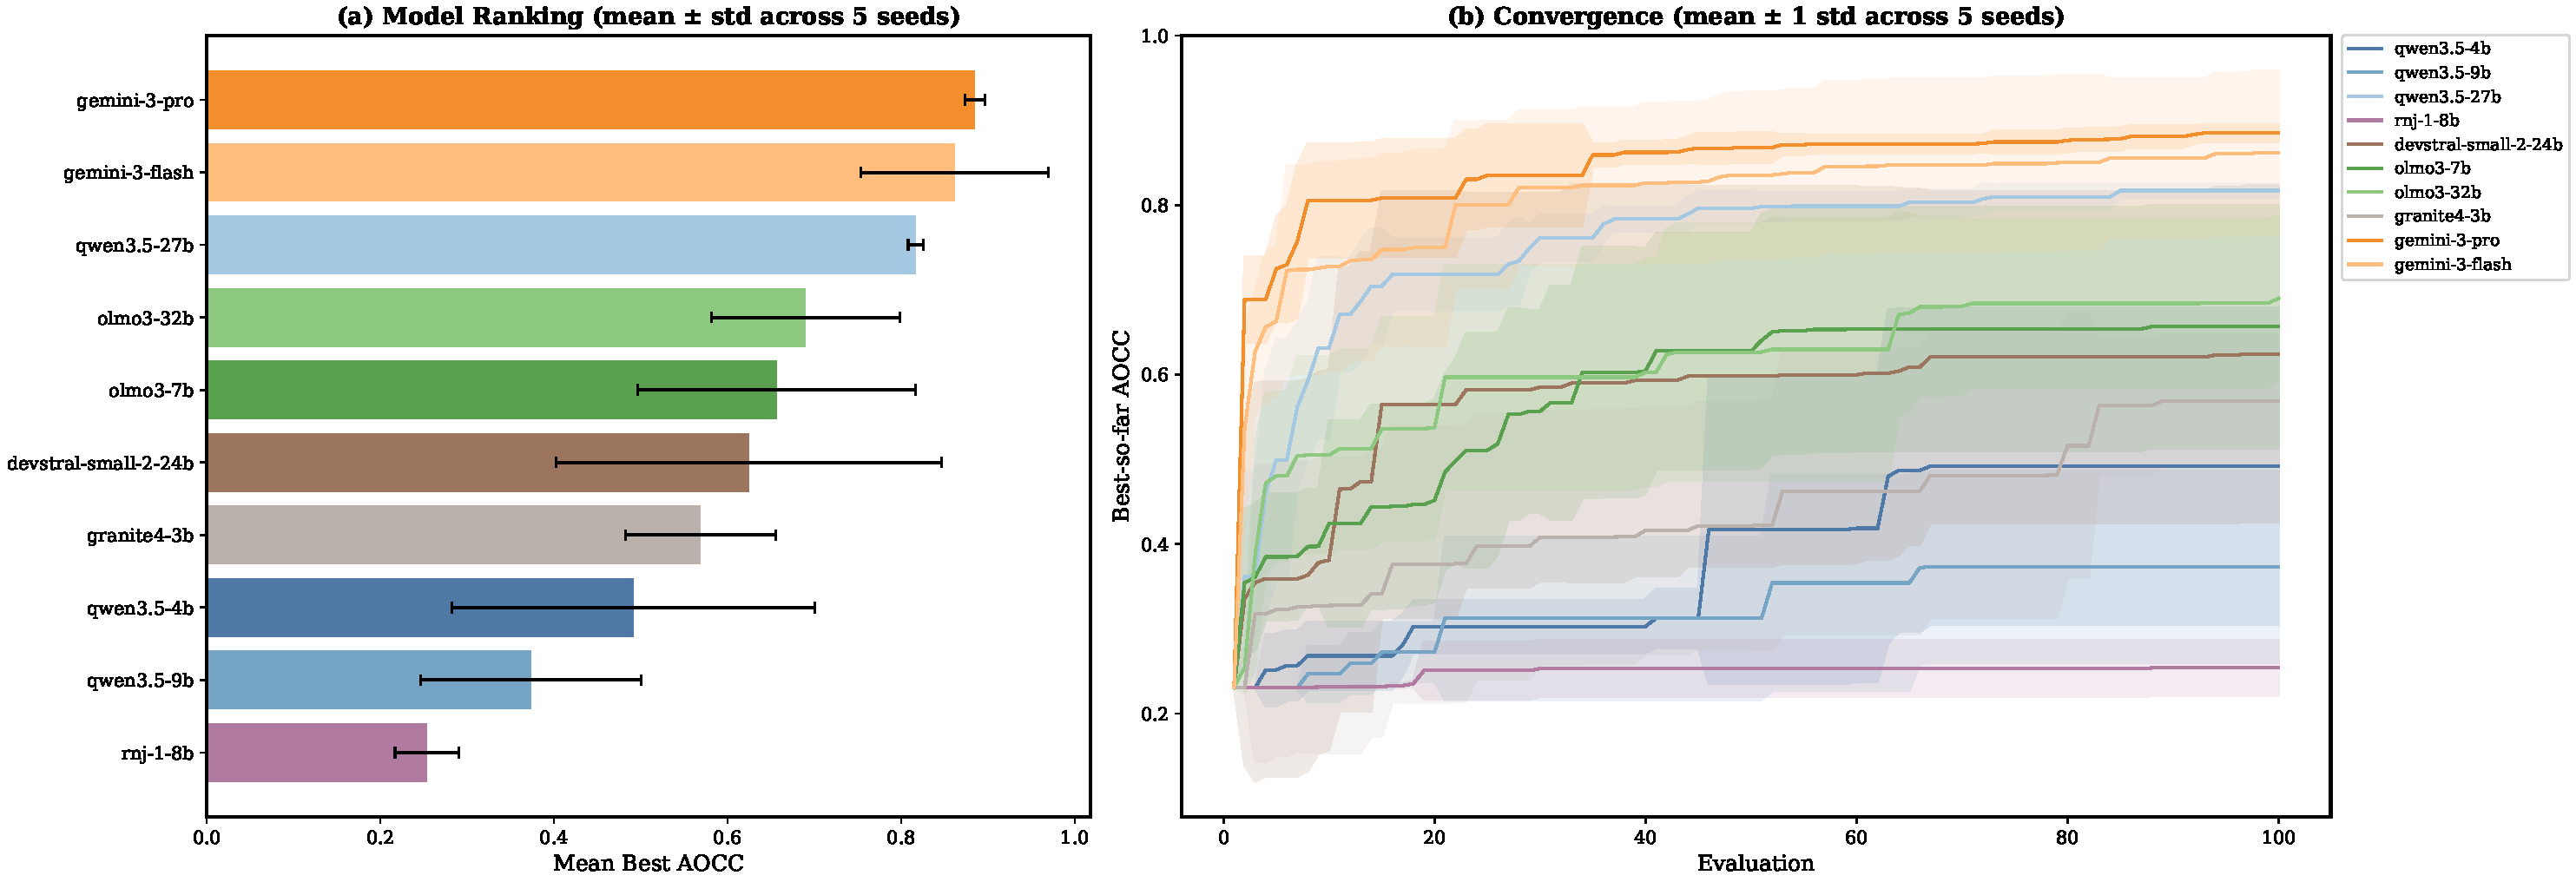
\includegraphics[width=\textwidth]{figures/fig_model_screening.pdf}
  \caption{LLM screening results. (a)~Mean best AOCC by model ($\pm$ std across 5 seeds). (b)~Best-so-far AOCC over 100 evaluations, averaged across 5 seeds. Shaded regions show $\pm$1 std.}
  \label{fig:model-screening}
\end{figure*}

This chapter reports the experimental outcomes of the four-stage pipeline described in \cref{ch:methodology}. \Cref{sec:results-screening} ranks the ten candidate LLMs and identifies the model carried into later stages. \Cref{sec:results-features} reduces the 32 behavioural features to a tractable, predictive subset. \Cref{sec:results-feedback} compares the three feedback framings of those features against the vanilla baseline. \Cref{sec:results-stage4} runs the head-to-head comparison of vanilla, neutral-behavioural, SAGE, and combined feedback on the twenty-function MA-BBOB set with longer evolutionary runs and more independent seeds.

% ===========================================================================
\section{LLM Screening}
\label{sec:results-screening}

\Cref{tab:model-ranking} presents the performance ranking of all 10 models, sorted by mean best AOCC across 5 seeds. The API models clearly dominate. Gemini~3 Pro achieves the highest mean best AOCC of $0.885 \pm 0.011$ with high consistency across seeds, while Gemini~3 Flash follows closely at $0.862$ with the lowest failure rate of any model at just $2.0\%$. The convergence curves in \cref{fig:model-screening}b show that Gemini models improve steadily throughout the full 100-evaluation budget, whereas most open-weight models plateau early or stagnate after initial gains.

\begin{table}[t]
\centering
\caption{Stage~1 model ranking (100 candidates $\times$ 5 seeds, vanilla feedback). Fail\% and AOCC averaged across seeds ($\pm$ std).}
\label{tab:model-ranking}
\footnotesize
\begin{tabular}{@{}rlrrr@{}}
\toprule
\textbf{\#} & \textbf{Model} & \textbf{Fail\%} & \textbf{AOCC} & \textbf{h/run} \\
\midrule
1  & Gem.~3 Pro    & 10.2  & .885$\pm$.011 & 5.1 \\
2  & Gem.~3 Flash  & \textbf{2.0} & .862$\pm$.108 & 3.9 \\
3  & Qwen3.5 27B   & 41.0  & .817$\pm$.009 & 38.9 \\
4  & OLMo~3 32B    & 13.2  & .690$\pm$.109 & 39.3 \\
5  & OLMo~3 7B     & 27.6  & .657$\pm$.160 & 18.4 \\
6  & Devstral~2    & 32.6  & .625$\pm$.222 & 5.0 \\
7  & Granite~4 3B  & 53.8  & .569$\pm$.087 & \textbf{0.6} \\
8  & Qwen3.5 4B    & 76.2  & .492$\pm$.209 & 7.9 \\
9  & Qwen3.5 9B    & 91.6  & .373$\pm$.127 & 3.0 \\
10 & RNJ-1 8B      & 34.6  & .254$\pm$.037 & 14.5 \\
\bottomrule
\end{tabular}
\end{table}


Among open-weight models, performance does not scale with parameter count. Qwen3.5~27B achieves $0.817$, outperforming the larger OLMo~3 32B at $0.690$. Granite~4, the smallest model at just 3B parameters, reaches $0.569$ and outperforms both Qwen3.5~9B at $0.373$ and RNJ-1~8B at $0.254$. This suggests that code generation ability for optimisation algorithms depends more on training data and architecture than on raw scale. Failure rates vary dramatically, from $2.0\%$ for Gemini~3 Flash to $91.6\%$ for Qwen3.5~9B, which fails to produce a valid algorithm class in the vast majority of attempts. Wall-clock time also varies substantially. The two models served via vLLM, Granite~4 at 0.6\,h/run and Qwen3.5~9B at 3.0\,h/run, benefit from continuous batching that allows concurrent seed evaluation. The largest open-weight models, Qwen3.5~27B and OLMo~3 32B, require approximately 39 hours per run under Ollama due to both model size and serial request queuing.

\subsection{Failure Mode Analysis}
\label{sec:results-failures}

Across all 10 models and 5 seeds, 5{,}000 candidates were generated in total, of which $3{,}071$ or $61.4\%$ produced valid fitness scores. The nature of failures differs systematically between strong and weak models. The top performing Gemini models have the lowest failure rates and predominantly fail due to runtime errors, where the generated code has the correct class interface but contains logic bugs that cause exceptions during evaluation. Weaker models instead produce structural failures, generating standalone functions rather than the required Python class or omitting mandatory constructor parameters.


\begin{figure}[t]
  \centering
  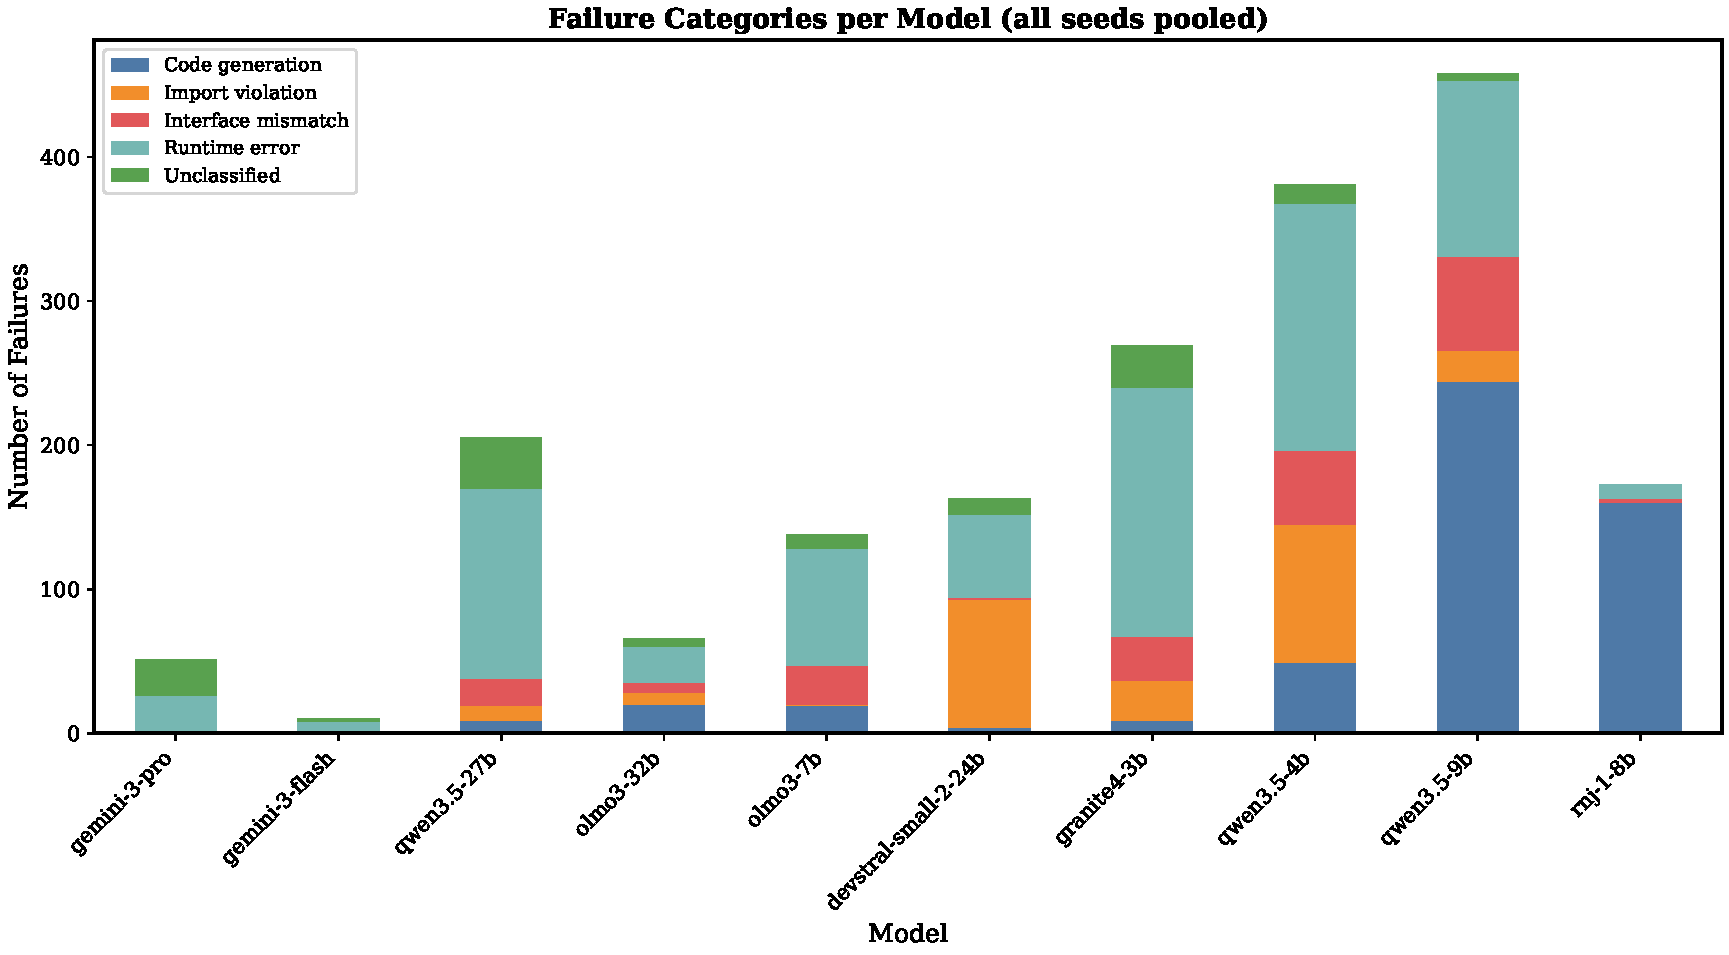
\includegraphics[width=\columnwidth]{figures/fig_failure_modes.pdf}
  \caption{Failure mode distribution by model. Categories include runtime errors (correct interface, logic bugs), structural failures (no class produced), and import errors.}
  \label{fig:failure-modes}
\end{figure}

\subsection{Behavioural Space}
\label{sec:results-behavioural-space}

\begin{figure*}[t]
  \centering
  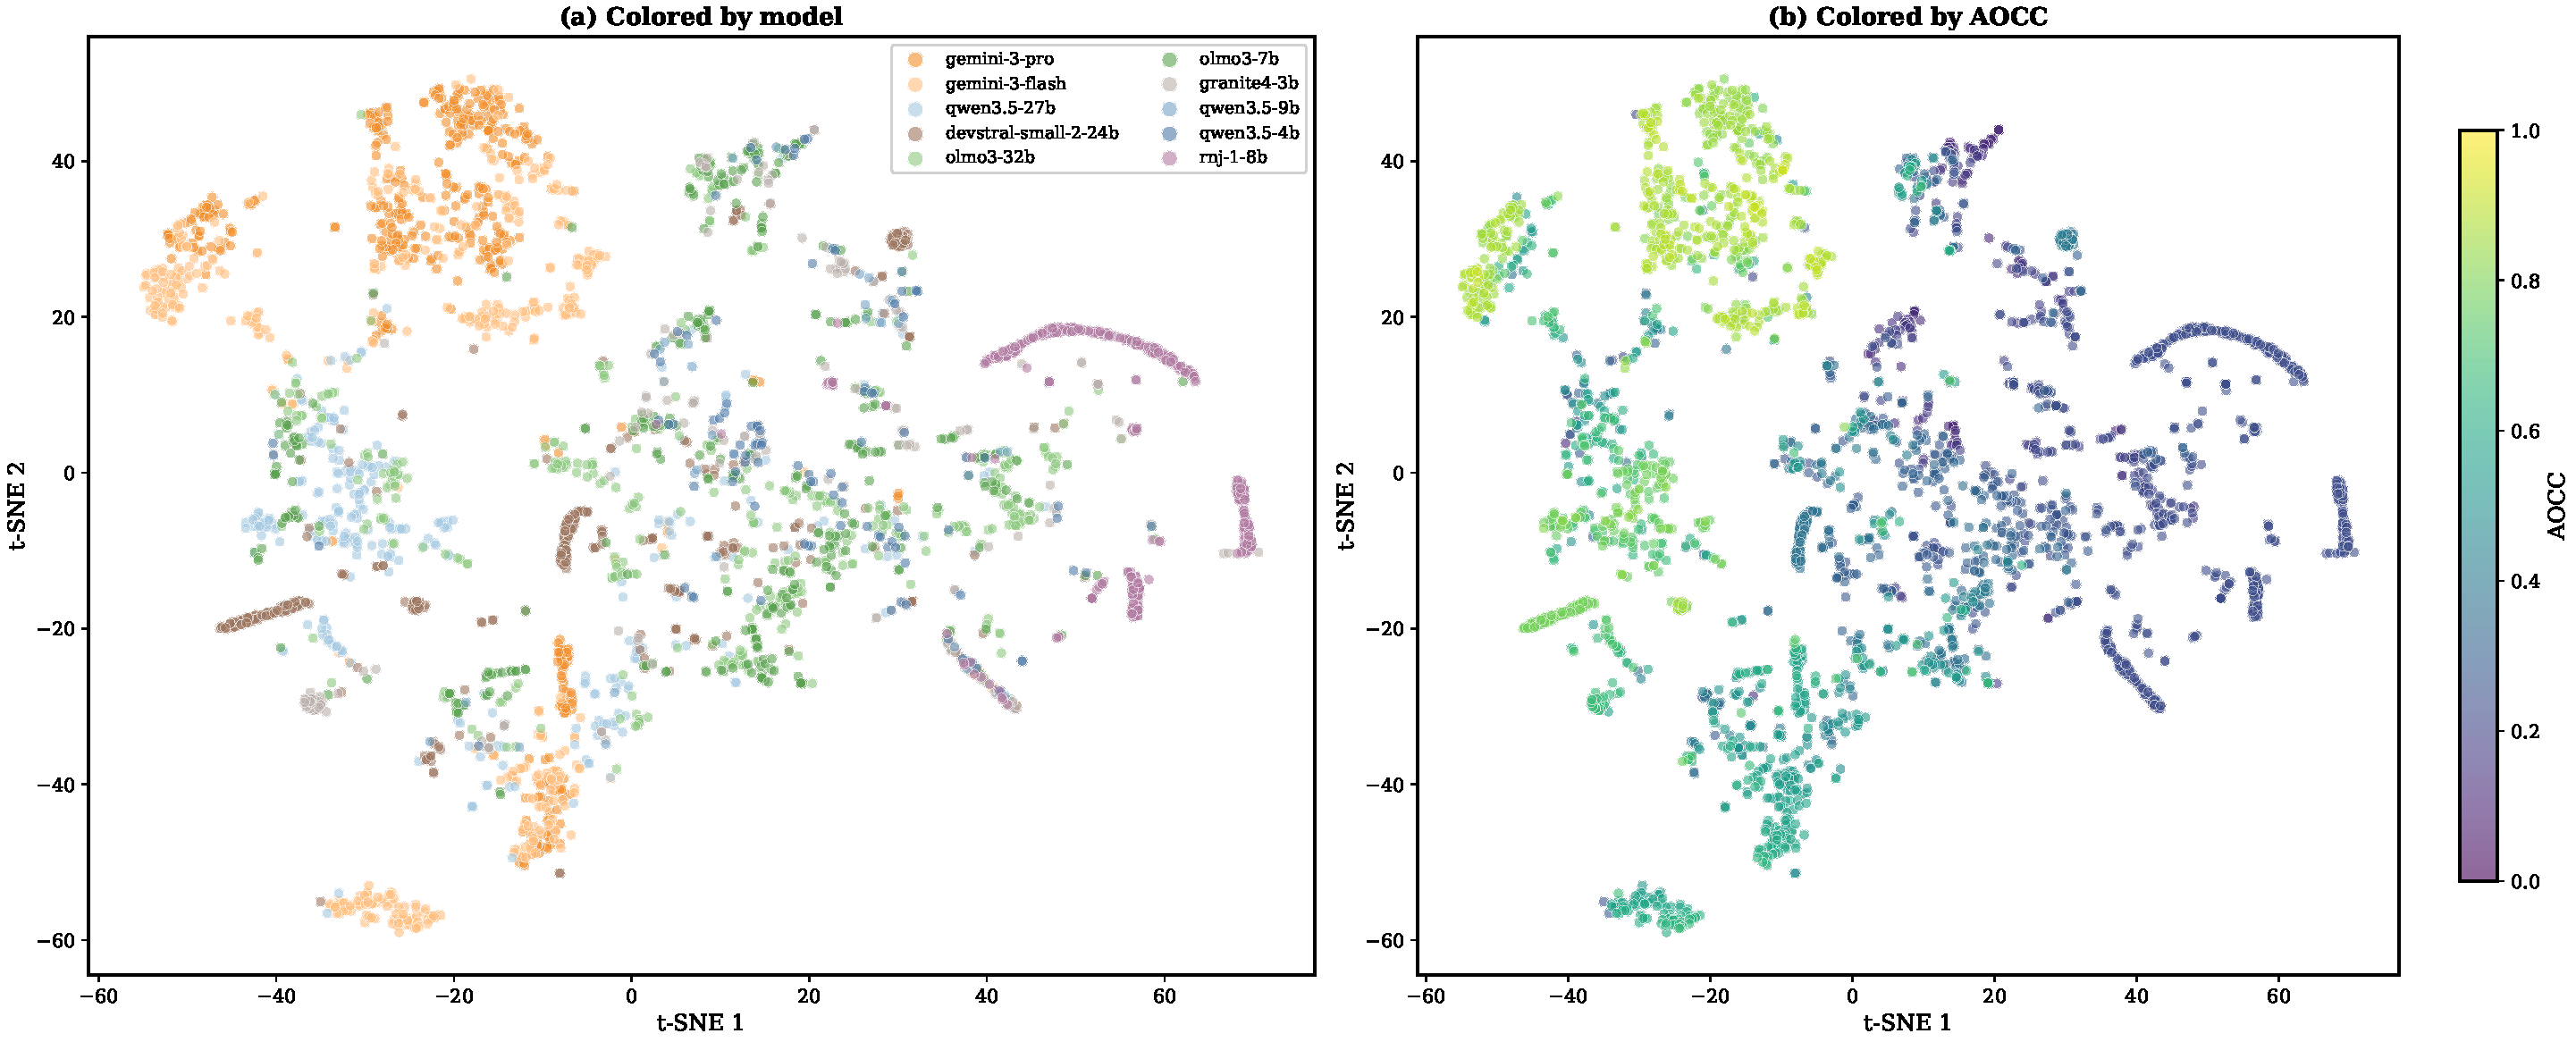
\includegraphics[width=\textwidth]{figures/fig_tsne_behavioral.pdf}
  \caption{t-SNE projection of the behavioural feature space for all $3{,}071$ valid algorithms. (a)~Points coloured by model reveal distinct clustering. Each LLM occupies a characteristic region, with some models forming elongated trajectories indicating incremental refinement. (b)~Points coloured by AOCC show that high-performing algorithms (yellow) concentrate in specific regions, while low-performing ones (purple) spread diffusely.}
  \label{fig:tsne-behavioral}
\end{figure*}

\begin{figure}[p]
  \centering
  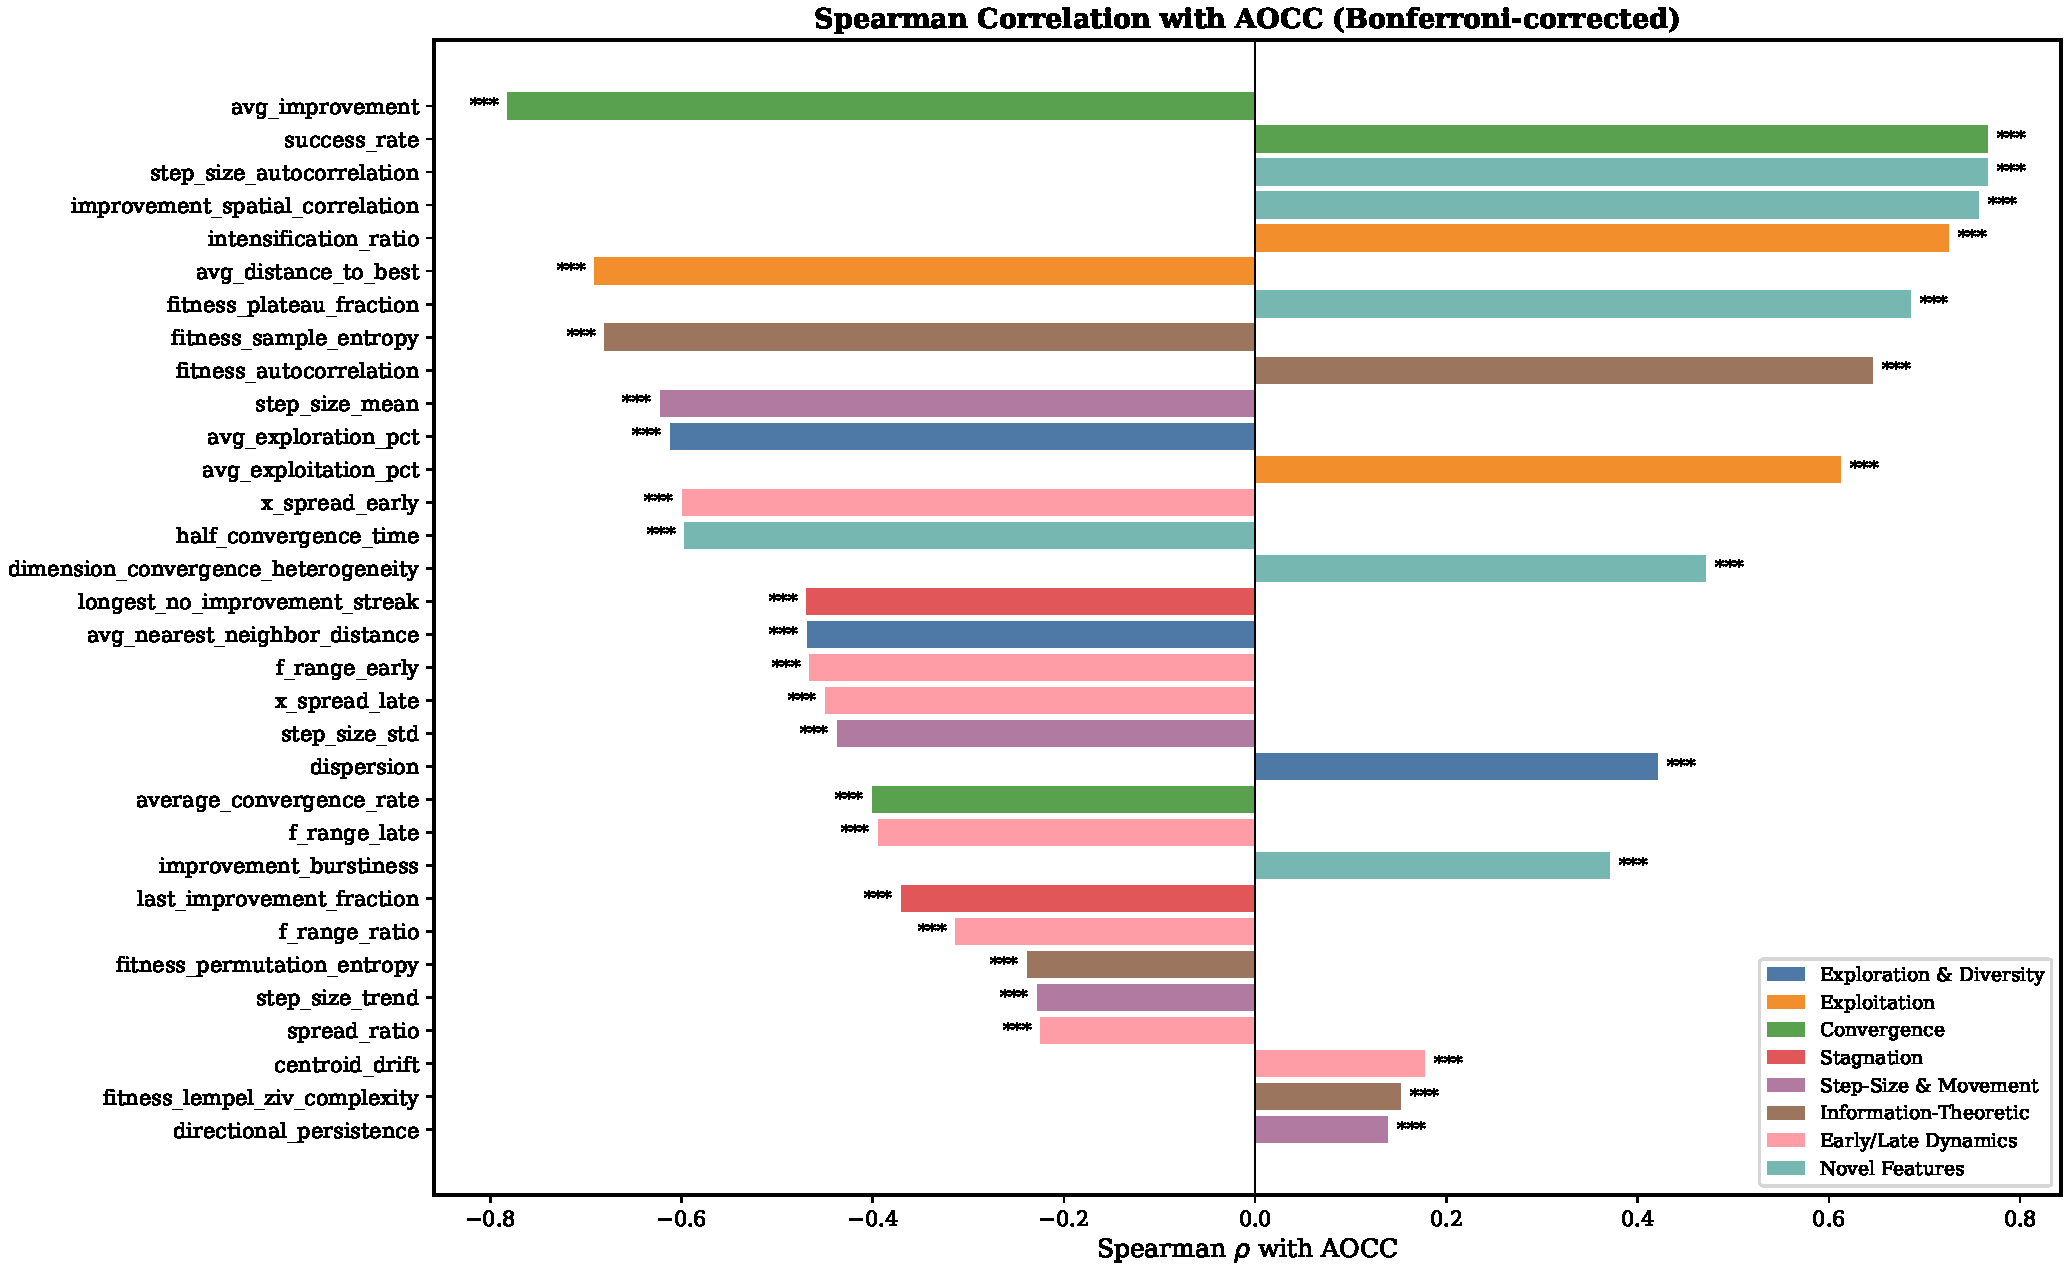
\includegraphics[width=\columnwidth]{figures/fig_spearman.pdf}
  \caption{Spearman rank correlation $\rho$ between each behavioural feature and AOCC across all $3{,}071$ valid candidates, sorted by $|\rho|$ and coloured by feature category. All features significant at $p < 0.001$ after Bonferroni correction.}
  \label{fig:spearman}
\end{figure}

\Cref{fig:tsne-behavioral} projects all valid candidates into a two-dimensional behavioural space via t-SNE on the 32 standardised features. Several patterns emerge. First, algorithms from the same model cluster together, confirming that each LLM produces a characteristic behavioural signature. The Gemini models dominate the upper-left quadrant, which panel~(b) reveals as the high-AOCC region (predominantly yellow-green). Second, several models produce elongated, chain-like trajectories rather than round clusters. RNJ-1 (right side) shows this most clearly, forming distinct arcs that trace the $(1+1)$-ES refinement path through behavioural space. Third, some models fragment into multiple sub-clusters, corresponding to different seeds exploring distinct algorithmic strategies. Fourth, the highest-performing algorithms from open-weight models (Qwen3.5~27B, OLMo~32B) partially overlap with the Gemini cluster, suggesting that strong optimisation behaviour converges to similar behavioural profiles regardless of the generating model. Weaker models (RNJ-1, Qwen3.5~4B) are confined to peripheral, low-AOCC regions with no overlap.

\subsection{Model Selection}
\label{sec:results-model-selection}

Gemini~3 Flash is selected for future experiments based on its combination of competitive AOCC ($0.862$), lowest failure rate ($2.0\%$), and fast inference (3.9h/run). Its vanilla performance across 5 seeds ($0.862 \pm 0.097$) serves as the baseline for all Stage~3 comparisons.

% ===========================================================================

\section{Feature Analysis and Selection}
\label{sec:results-features}

The Stage~1 dataset contains $3{,}071$ valid candidates. Each is accompanied by a 32-dimensional behavioural feature vector computed from its evaluation trajectory. This section determines which features are most predictive of algorithm quality and selects a tractable subset for the feedback experiments.

\subsection{Feature--AOCC Correlations}
\label{sec:results-correlations}

\Cref{fig:spearman} shows the Spearman rank correlation between each of the 32 behavioural features and AOCC. Given the sample size, all 32 correlations are statistically significant at $p < 0.001$ after Bonferroni correction, so significance is not a useful discriminator. Instead, we focus on the magnitude and direction of $\rho$ to understand which behaviours characterise high-performing algorithms.

The five strongest associations are \texttt{avg\_improvement} ($-0.782$), \texttt{success\_rate} ($+0.766$), \texttt{step\_size\_autocorrelation} ($+0.766$), \texttt{improvement\_spatial\_correlation} ($+0.757$), and \texttt{intensification\_ratio} ($+0.725$). Three of these five are introduced to LLaMEA-generated metaheuristic analysis in this thesis.

Examining correlations by feature category reveals a clear behavioural profile of successful algorithms. The \emph{exploitation} features show the strongest positive associations. High \texttt{intensification\_ratio} ($+0.725$) and low \texttt{avg\_distance\_to\_best} ($-0.691$) indicate that good algorithms focus their search near the best-known solution. The \emph{convergence} features reinforce this picture. Low \texttt{avg\_improvement} ($-0.782$) means the algorithm has already found good solutions early, leaving less room for further gains, while high \texttt{fitness\_plateau\_fraction} ($+0.685$) reflects spending more of the budget in a converged state. Among the \emph{step-size and movement} features, \texttt{step\_size\_autocorrelation} ($+0.766$) stands out, indicating that smooth, momentum-driven step sizes outperform erratic adjustments. The \emph{early/late dynamics} features confirm that successful algorithms do not waste early evaluations on broad exploration. \texttt{x\_spread\_early} ($-0.599$) shows that narrower initial search correlates with higher AOCC. In contrast, the \emph{exploration} features show moderate negative correlations ($|\rho| \approx 0.4$--$0.6$), suggesting that excessive diversity is counterproductive on this benchmark. The weakest associations appear among structural features such as \texttt{directional\_persistence} ($+0.139$) and \texttt{fitness\_lempel\_ziv\_complexity} ($+0.152$), which capture trajectory properties largely uncorrelated to AOCC.

\subsection{Predictive Power}
\label{sec:results-rf}

To capture non-linear and interaction effects that Spearman correlation misses, a Random Forest regressor with 200 trees is trained on all 32 features to predict AOCC. The model achieves an out-of-bag $R^2$ of $0.962$ and a mean absolute error of $0.024$ AOCC units. The $R^2$ indicates that 96.2\% of the variance in AOCC across candidates is explained by their behavioural features, while the MAE means the model's predictions are off by just 0.024 on average. This tight fit is expected because the features are computed from the same evaluation trajectory that determines AOCC. They are not independent predictors but rather complementary summaries of the underlying search dynamics.

\Cref{fig:rf-importance} shows the permutation importance ranking. While the same features appear near the top as in the Spearman analysis, the relative weighting differs notably. \texttt{avg\_improvement} ($0.291$) and \texttt{fitness\_plateau\_fraction} ($0.215$) account for the majority of predictive power, far exceeding the third-ranked \texttt{success\_rate} ($0.107$). This concentration suggests that convergence behaviour, specifically how quickly and completely an algorithm reaches a plateau, is the single most important determinant of AOCC. In contrast, \texttt{step\_size\_autocorrelation}, which ranks third by Spearman $|\rho|$, drops to rank 10 by importance. This indicates that while smooth step sizes correlate with quality, their predictive value is largely captured by other features in the ensemble. The RF ranking also elevates \texttt{average\_convergence\_rate} (rank 6) and \texttt{fitness\_permutation\_entropy} (rank 5), features with moderate Spearman correlations but apparently strong non-linear predictive power.

\begin{figure}[p]
  \centering
  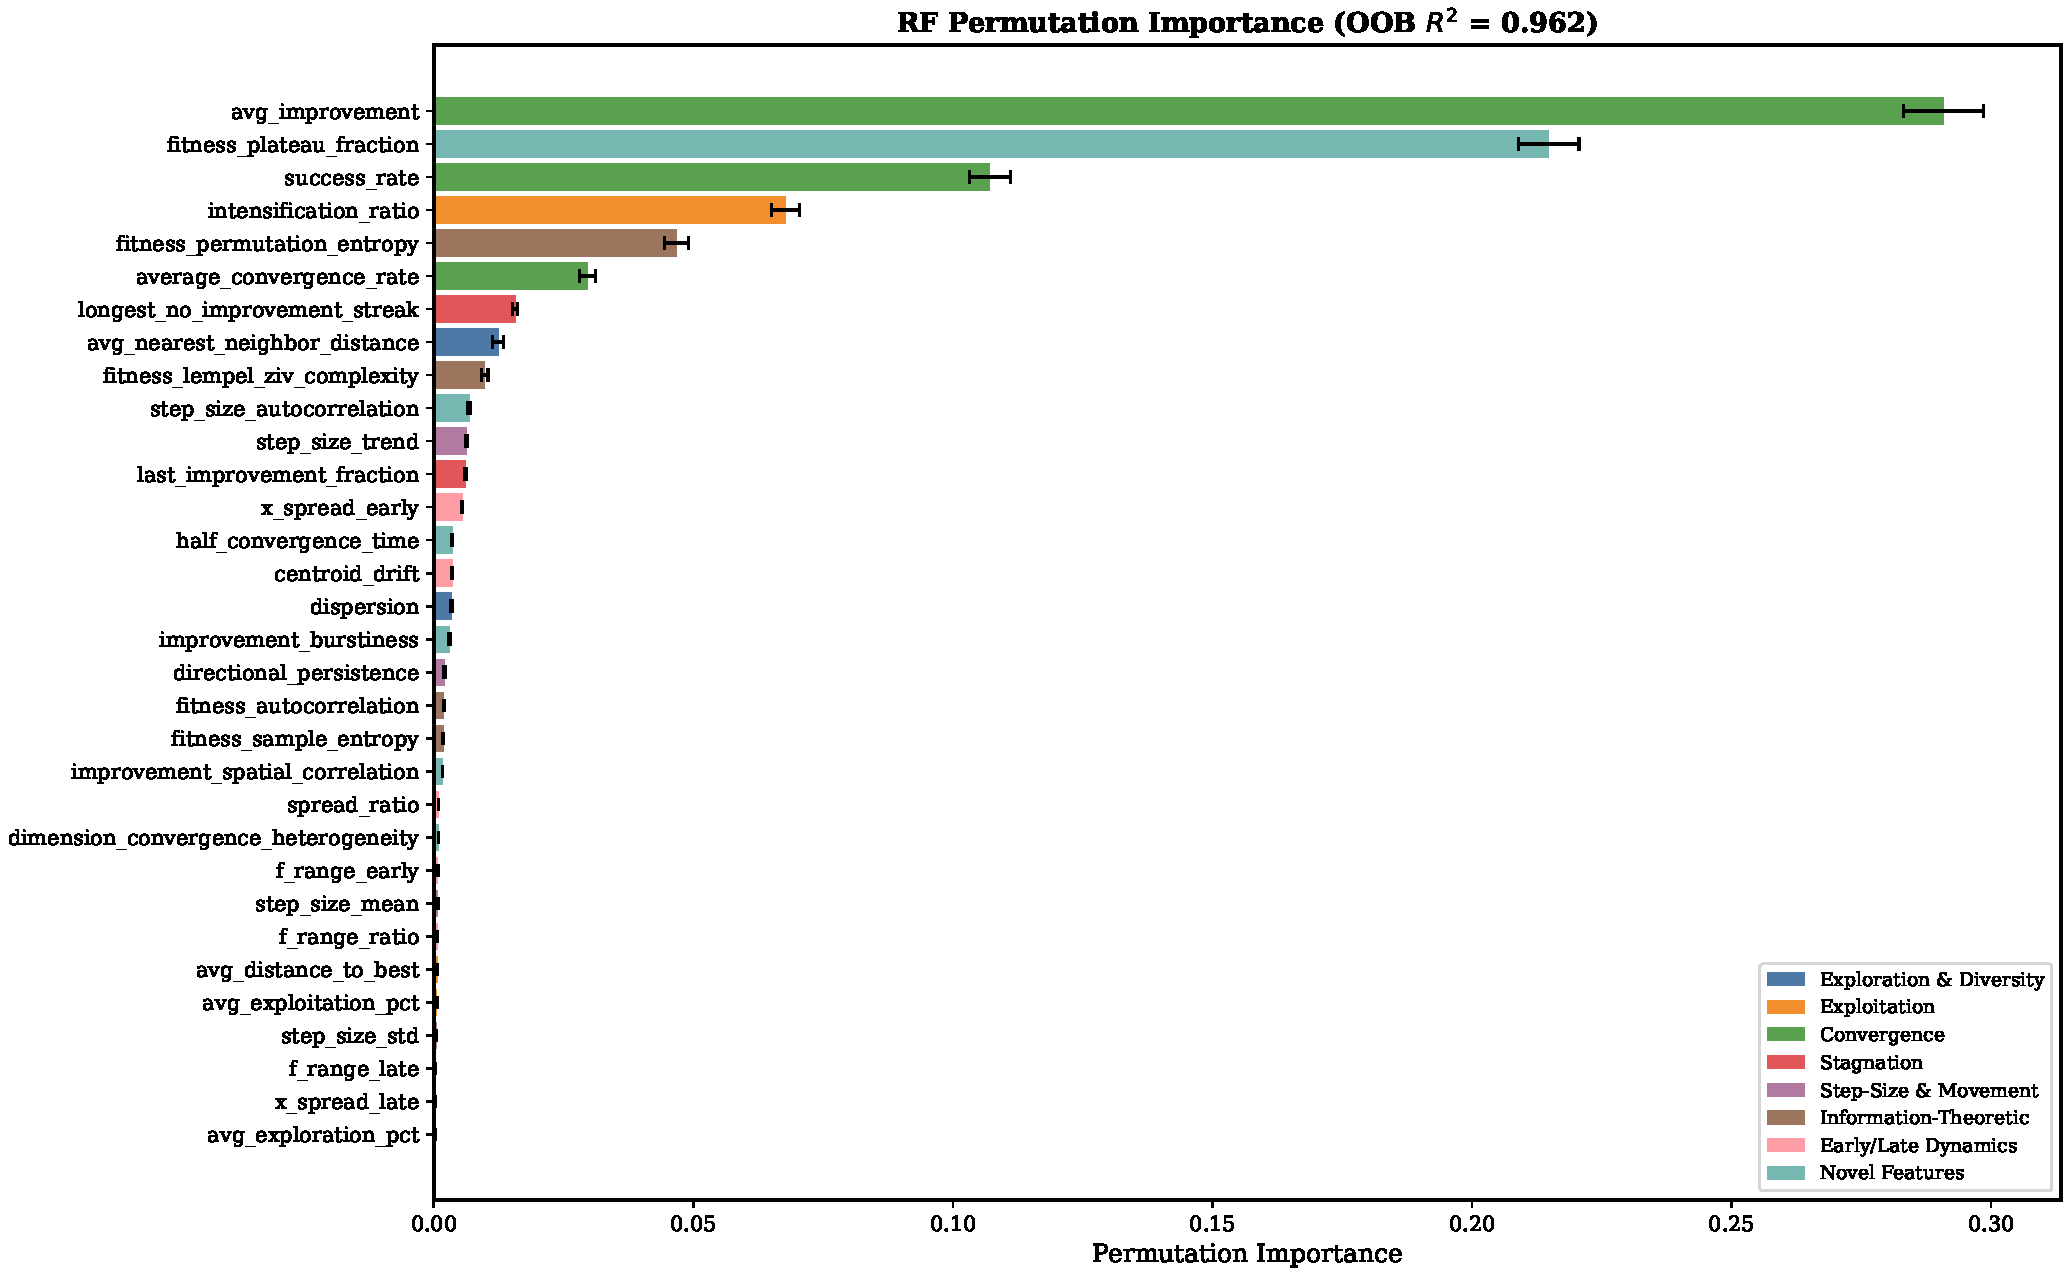
\includegraphics[width=\columnwidth]{figures/fig_rf_importance.pdf}
  \caption{Random Forest permutation importance for all 32 features, sorted by importance. Error bars show standard deviation across 10 permutation repeats.}
  \label{fig:rf-importance}
\end{figure}

\begin{figure}[p]
  \centering
  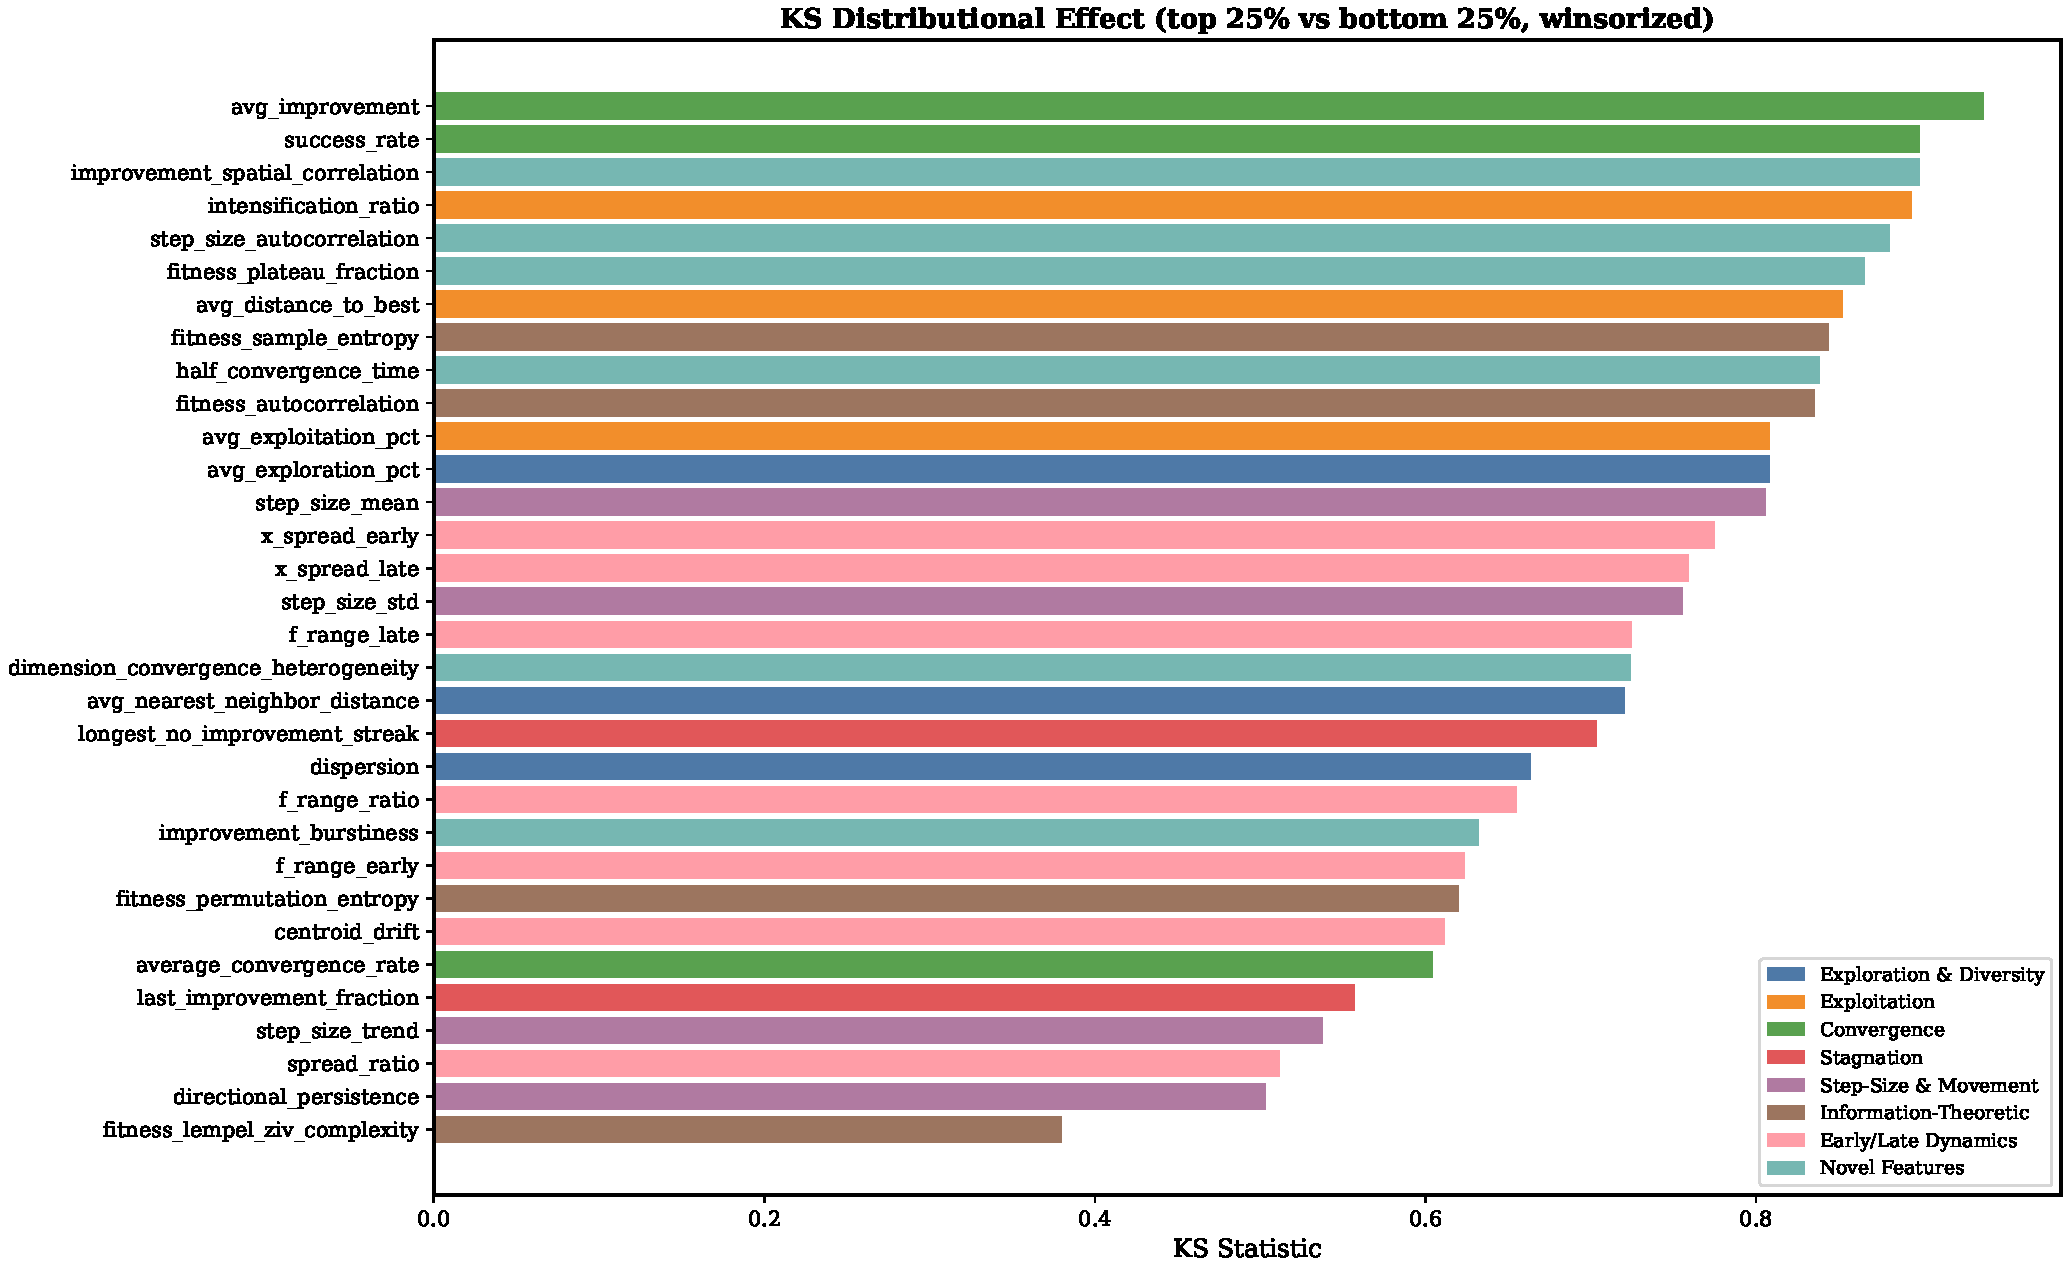
\includegraphics[width=\columnwidth]{figures/fig_ks_effect.pdf}
  \caption{KS distributional effect size between top-25\% and bottom-25\% algorithms by AOCC, sorted by KS statistic. Feature values are winsorized at the 1st/99th percentile before testing.}
  \label{fig:ks-effect}
\end{figure}

\subsection{Distributional Separation}
\label{sec:results-ks}

\Cref{fig:ks-effect} reports the KS statistic for each feature across the $3{,}071$ valid candidates. The KS ranking largely agrees with Spearman on which features matter most, but reveals additional structure. Several features that ranked moderately by Spearman show very high KS values, indicating they separate good from bad algorithms through non-monotonic or threshold effects rather than smooth linear trends. For example, \texttt{avg\_exploitation\_pct} and \texttt{step\_size\_mean} both achieve KS statistics above 0.8 despite more moderate Spearman $|\rho|$ values. At the bottom of the KS ranking, features like \texttt{fitness\_lempel\_ziv\_complexity} and \texttt{spread\_ratio} show weak distributional separation, confirming that they carry little information about algorithm quality regardless of the statistical method used.

\subsection{Consensus Ranking and Selection}
\label{sec:results-selection}

\begin{figure}[!t]
  \centering
  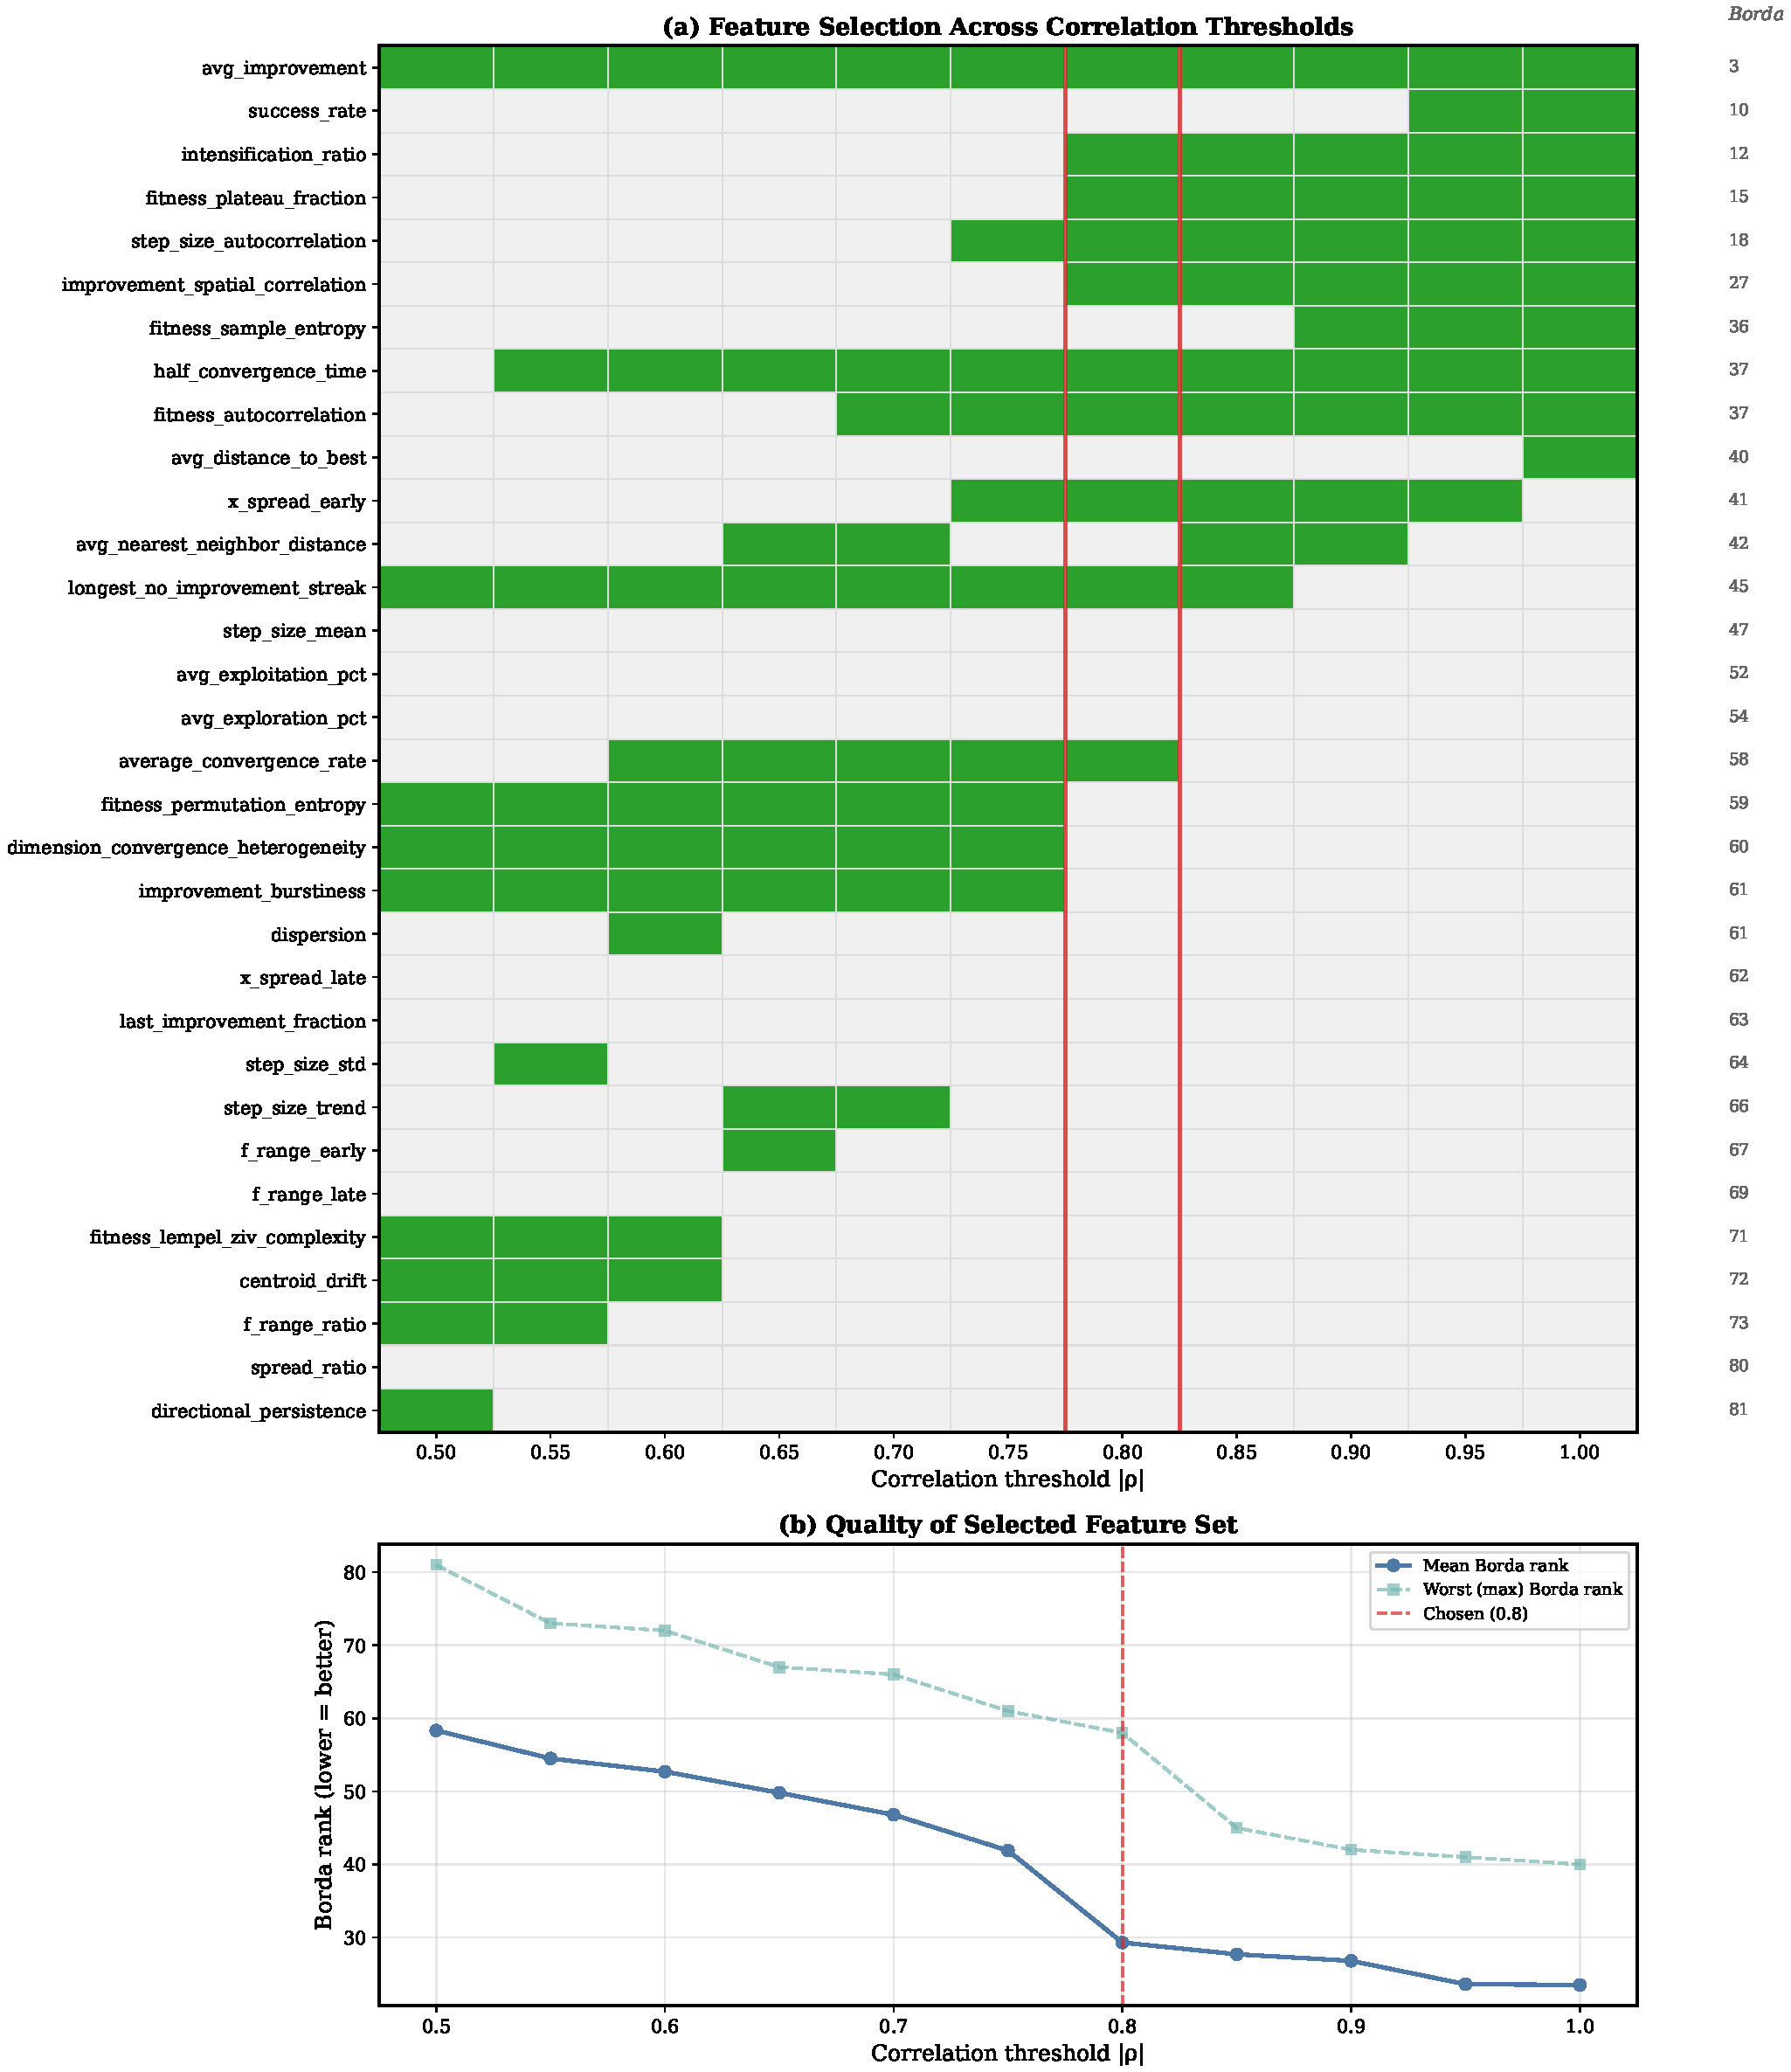
\includegraphics[width=\columnwidth]{figures/fig_feature_sensitivity_combined.pdf}
  \caption{Sensitivity of the 10-feature subset to the redundancy-pruning threshold $\tau$. (a)~Presence heatmap: which of the 32 candidates is selected at each $\tau \in [0.50, 1.00]$ in $0.05$ steps, sorted top-to-bottom by Borda rank. The chosen $\tau = 0.80$ column is highlighted in red. (b)~Mean and worst Borda rank of the selected subset as $\tau$ varies; the dashed line marks the chosen value, which sits at the elbow of the mean curve.}
  \label{fig:feature-sensitivity}

  \vspace{1em}
  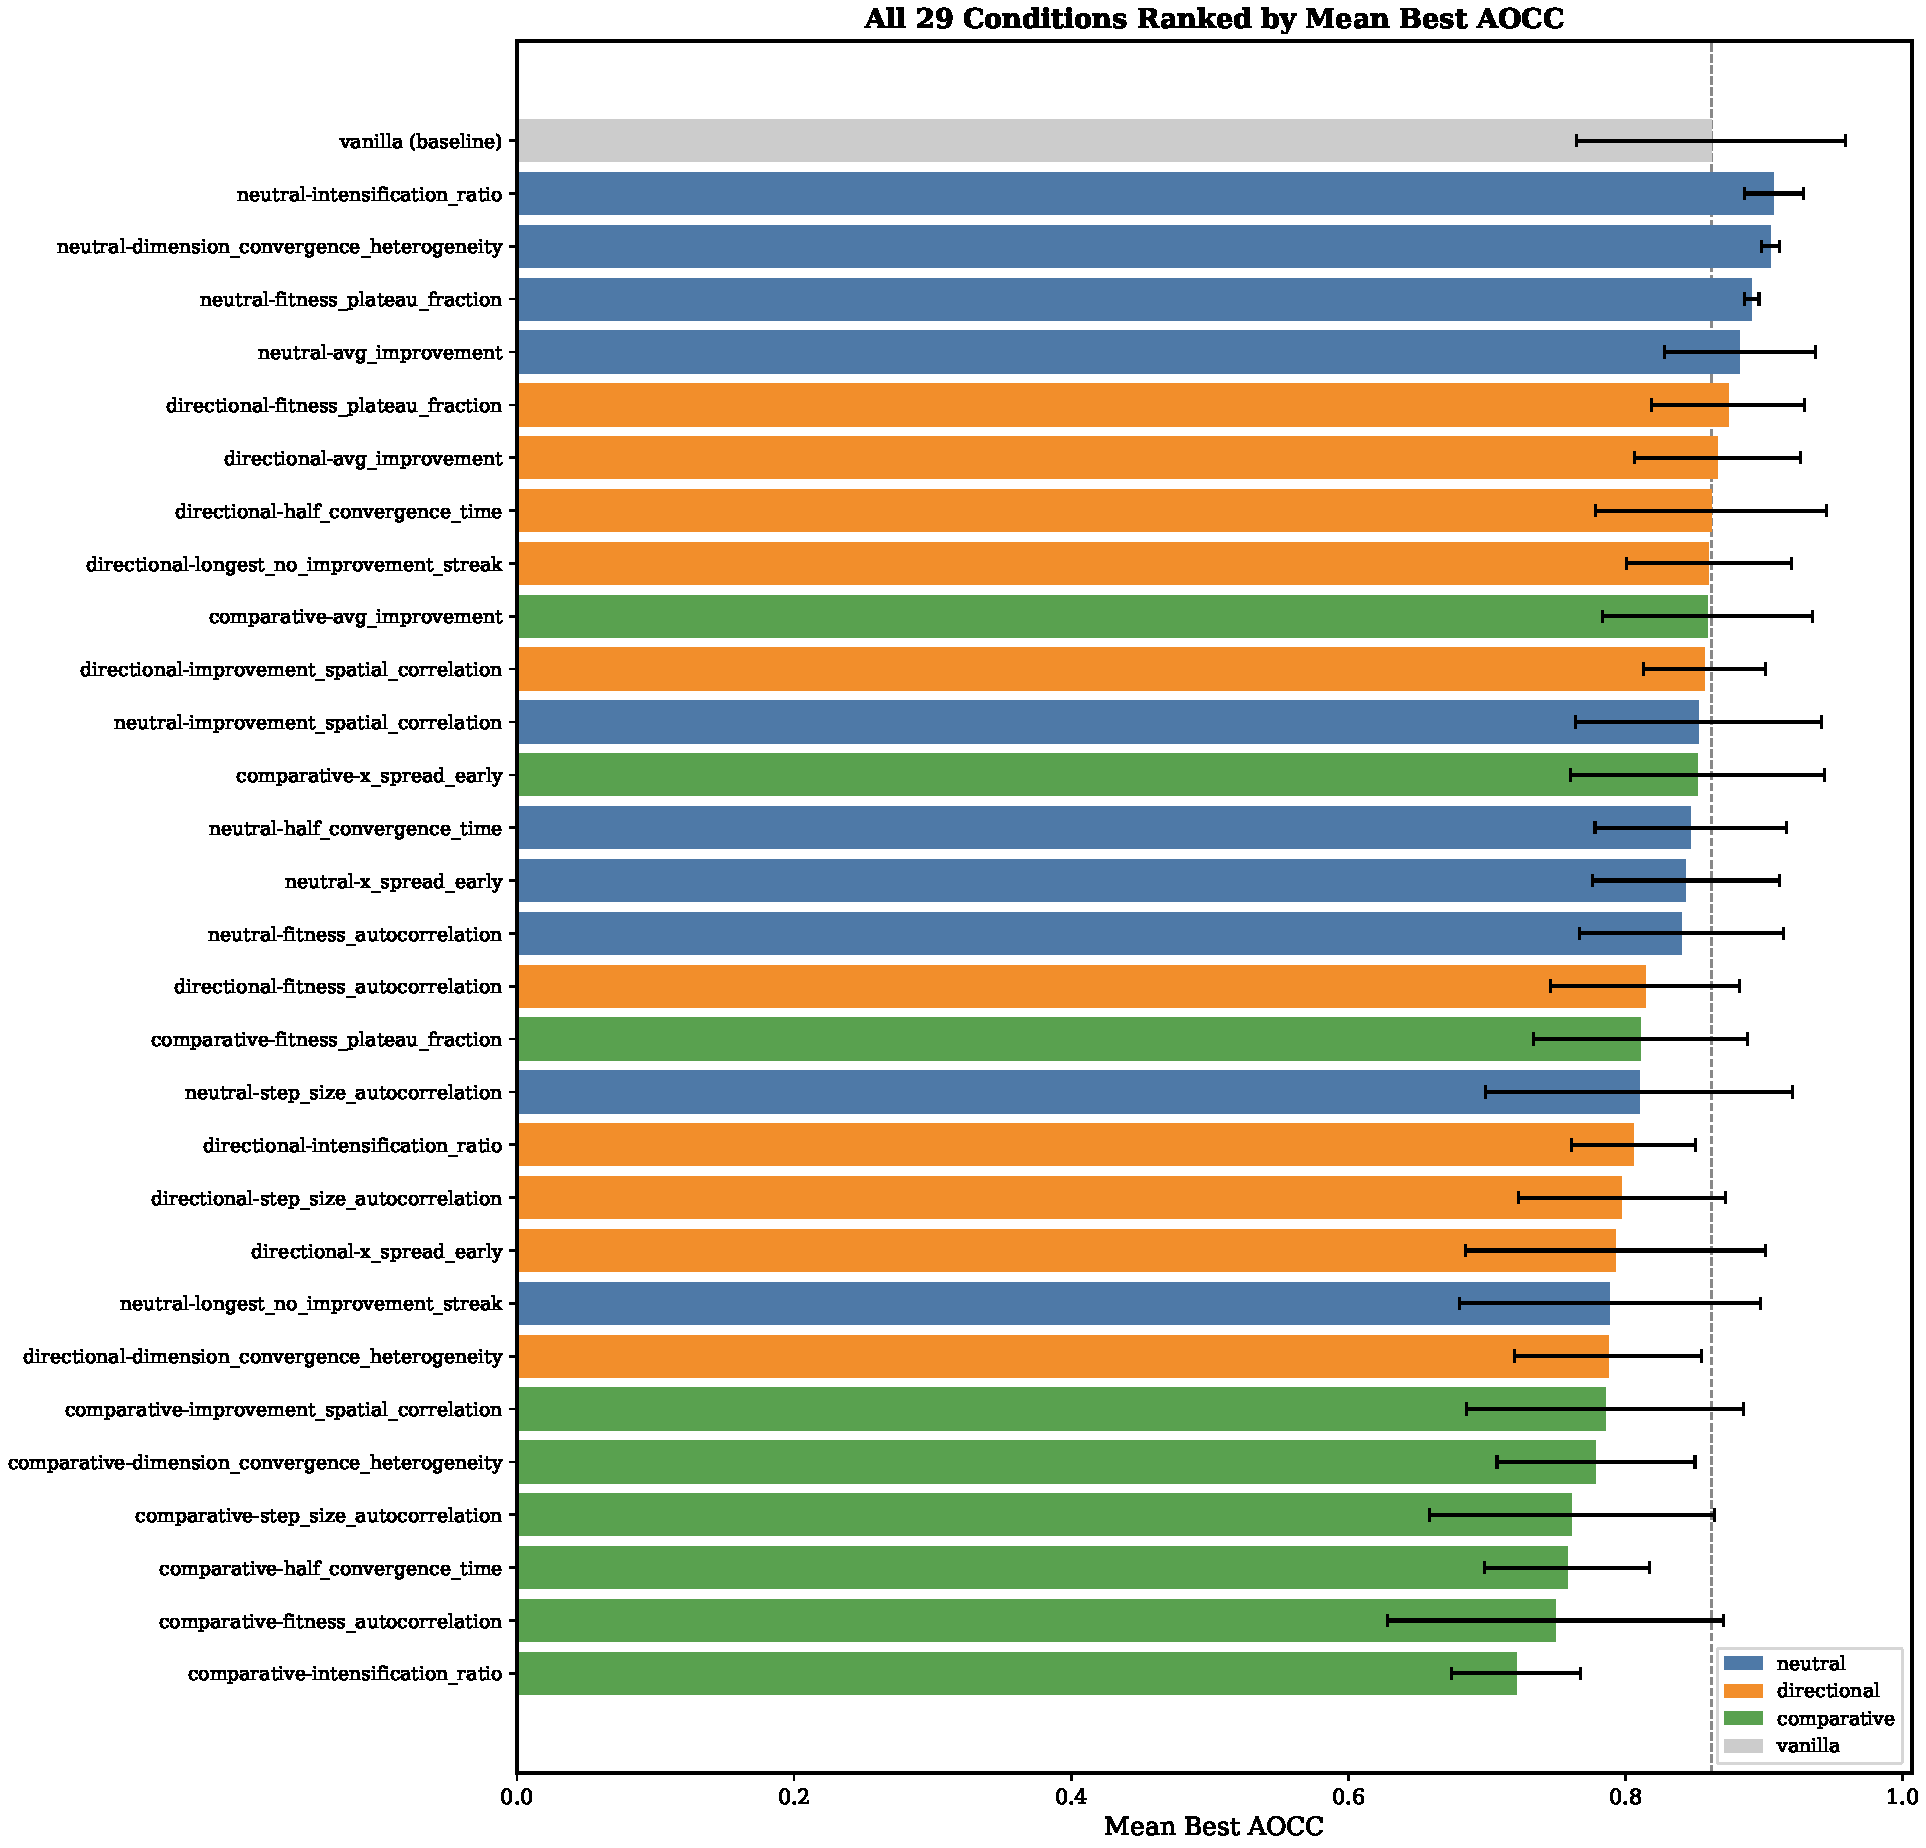
\includegraphics[width=\columnwidth]{figures/fig_condition_ranking.pdf}
  \caption{All 29 conditions ranked by mean best AOCC ($\pm$ std, 5 seeds). Grey bar and dashed line show the vanilla baseline ($0.862$). Colours: blue = neutral, orange = directional, green = comparative.}
  \label{fig:condition-ranking}
\end{figure}

\begin{table*}[p]
\centering
\caption{All 32 behavioural features ranked by Borda consensus. For each method, both the value and rank are shown. The Status column indicates whether a feature was selected for feedback experiments, pruned for redundancy (with the correlated selected feature noted), or not selected.}
\label{tab:feature-consensus}
\footnotesize
\setlength{\tabcolsep}{3.5pt}
\begin{tabular}{@{}rlrrrrrrl@{}}
\toprule
& & \multicolumn{2}{c}{\textbf{Spearman}} & \multicolumn{2}{c}{\textbf{RF Importance}} & \multicolumn{2}{c}{\textbf{KS}} & \\
\cmidrule(lr){3-4} \cmidrule(lr){5-6} \cmidrule(lr){7-8}
\textbf{Borda} & \textbf{Feature} & \boldmath{$\rho$} & \textbf{R} & \textbf{Imp} & \textbf{R} & \textbf{Stat} & \textbf{R} & \textbf{Status} \\
\midrule
3  & avg\_improvement              & $-$.782 &  1 & .291 &  1 & .938 &  1 & \textbf{Selected} \\
7  & success\_rate                 & $+$.766 &  2 & .107 &  3 & .899 &  2 & Pruned ($|r|{=}.92$, avg\_impr) \\
13 & intensification\_ratio        & $+$.725 &  5 & .068 &  4 & .894 &  4 & \textbf{Selected} \\
15 & fitness\_plateau\_frac        & $+$.685 &  7 & .215 &  2 & .867 &  6 & \textbf{Selected} \\
18 & step\_size\_autocorr          & $+$.766 &  3 & .007 & 10 & .881 &  5 & \textbf{Selected} \\
28 & impr\_spatial\_corr           & $+$.757 &  4 & .002 & 21 & .899 &  3 & \textbf{Selected} \\
36 & fitness\_sample\_entropy      & $-$.680 &  8 & .002 & 20 & .845 &  8 & Pruned ($|r|{=}.87$, plateau\_frac) \\
37 & half\_convergence\_time       & $-$.597 & 14 & .004 & 14 & .840 &  9 & \textbf{Selected} \\
38 & fitness\_autocorrelation      & $+$.645 &  9 & .002 & 19 & .835 & 10 & \textbf{Selected} \\
40 & avg\_distance\_to\_best       & $-$.691 &  6 & .001 & 27 & .852 &  7 & Pruned ($|r|{=}.96$, intens\_ratio) \\
40 & x\_spread\_early              & $-$.599 & 13 & .006 & 13 & .775 & 14 & \textbf{Selected} \\
43 & longest\_no\_improv\_streak   & $-$.469 & 16 & .016 &  7 & .703 & 20 & \textbf{Selected} \\
44 & avg\_nn\_distance             & $-$.469 & 17 & .012 &  8 & .720 & 19 & Pruned ($|r|{=}.82$, x\_spread) \\
48 & step\_size\_mean              & $-$.622 & 10 & .001 & 25 & .806 & 13 & Pruned ($|r|{=}.83$, intens\_ratio) \\
52 & avg\_exploitation\_pct        & $+$.612 & 12 & .001 & 28 & .808 & 12 & Pruned ($|r|{=}.87$, intens\_ratio) \\
55 & avg\_exploration\_pct         & $-$.612 & 11 & .000 & 32 & .808 & 12 & Pruned ($|r|{=}.87$, intens\_ratio) \\
55 & dim\_conv\_heterogeneity      & $+$.471 & 15 & .001 & 23 & .727 & 17 & \textbf{Selected} \\
\midrule
55 & average\_convergence\_rate    & $-$.400 & 22 & .030 &  6 & .604 & 27 & --- \\
57 & fitness\_perm\_entropy        & $-$.238 & 27 & .047 &  5 & .622 & 25 & --- \\
58 & dispersion                    & $+$.421 & 21 & .003 & 16 & .664 & 21 & --- \\
64 & improvement\_burstiness       & $+$.370 & 24 & .003 & 17 & .635 & 23 & --- \\
65 & last\_improvement\_frac       & $-$.370 & 25 & .006 & 12 & .555 & 28 & --- \\
65 & step\_size\_std               & $-$.437 & 20 & .001 & 29 & .755 & 16 & --- \\
65 & x\_spread\_late               & $-$.450 & 19 & .000 & 31 & .759 & 15 & --- \\
66 & f\_range\_early               & $-$.466 & 18 & .001 & 24 & .624 & 24 & --- \\
68 & step\_size\_trend             & $-$.228 & 28 & .006 & 11 & .538 & 29 & --- \\
71 & f\_range\_late                & $-$.394 & 23 & .000 & 30 & .724 & 18 & --- \\
71 & centroid\_drift               & $+$.177 & 30 & .004 & 15 & .612 & 26 & --- \\
72 & fitness\_lempel\_ziv          & $+$.152 & 31 & .010 &  9 & .380 & 32 & --- \\
74 & f\_range\_ratio               & $-$.313 & 26 & .001 & 26 & .654 & 22 & --- \\
81 & spread\_ratio                 & $-$.224 & 29 & .001 & 22 & .511 & 30 & --- \\
81 & directional\_persistence      & $+$.139 & 32 & .002 & 18 & .502 & 31 & --- \\
\bottomrule
\end{tabular}
\\[0.3em]
{\scriptsize Borda = sum of ranks (lower is better). R = rank within method. Values are rounded to 3 decimal places. Where features appear tied, ranks reflect the full-precision ordering. Features above the mid-rule were evaluated by the greedy selection and those below were not considered (10 slots already filled). Pruned features show $|r|$ with the correlated selected feature.}
\end{table*}

The redundancy-pruning threshold $\tau$ controls how aggressively the greedy walk discards features that correlate with already-selected ones, and \cref{fig:feature-sensitivity} shows what happens to the selected subset across the swept range $\tau \in [0.50, 1.00]$ at an intervals of $0.05$. The top panel reports which of the 32 candidates survives at each $\tau$, sorted by Borda rank. The bottom panel tracks the mean and worst Borda rank of the selected subset as $\tau$ varies. Top-ranked features remain stable across the full range, while features lower in the Borda order swap in and out with small threshold changes. Tightening past $\tau = 0.80$ admits lower-Borda candidates and inflates the worst Borda rank in the subset. Loosening below $\tau = 0.80$ prunes features that still carry complementary signal. The mean Borda rank shows its largest single-step improvement at the $0.75$ to $0.80$ transition and plateaus thereafter, motivating $\tau = 0.80$ as the elbow of the quality--threshold curve.

\Cref{tab:feature-consensus} presents all 32 features with their per-method values and ranks, sorted by Borda consensus score. The final set comprises three BLADE features and seven newly introduced features from this thesis, validating the feature design effort described in \cref{ch:features}. \Cref{tab:feature-consensus} reveals that \texttt{intensification\_ratio} alone makes four other metrics redundant, including two BLADE exploration/exploitation percentages and the widely used \texttt{avg\_distance\_to\_best}. Several features with strong individual method rankings fail the consensus. For example, \texttt{fitness\_permutation\_entropy} ranks 5th by RF importance but only 27th by Spearman.

% ===========================================================================
\section{Behavioural Feedback}
\label{sec:results-feedback}

The Stage~3 dataset contains $14{,}127$ valid candidates produced by Gemini~3 Flash across 29 feedback conditions (10 features $\times$ 3 framings, minus the comparative version of \texttt{longest\_no\_improvement\_streak} excluded for non-monotonicity) with 5 independent seeds per condition. This section compares the three feedback formats against each other and against the vanilla AOCC-only baseline, then examines how reliably each format steers behaviour toward the prescribed direction and how the underlying feature--AOCC signal shifts between Stage~1 and Stage~3.

\begin{table*}[!t]
\centering
\caption{Behavioural steering results per feature. For each format: mean best AOCC ($\pm$ std) and median behavioural feature value ($\pm$ std). The final columns show whether directional/comparative shifted the feature toward the advised direction relative to neutral.}
\label{tab:steering-detail}
\footnotesize
\setlength{\tabcolsep}{3.5pt}
\begin{tabular}{@{}lr|rr|rr|rr|cc@{}}
\toprule
& & \multicolumn{2}{c|}{\textbf{Neutral}} & \multicolumn{2}{c|}{\textbf{Directional}} & \multicolumn{2}{c|}{\textbf{Comparative}} & \multicolumn{2}{c}{\textbf{Steered}} \\
\textbf{Feature} & \textbf{Adv.} & \textbf{AOCC} & \textbf{Feat.} & \textbf{AOCC} & \textbf{Feat.} & \textbf{AOCC} & \textbf{Feat.} & \textbf{D} & \textbf{C} \\
\midrule
avg\_impr      & $\downarrow$ & \textbf{.883$\pm$.054} & .094$\pm$.198 & .866$\pm$.060 & .105$\pm$.206 & .860$\pm$.076 & .104$\pm$.237 & $\times$ & $\times$ \\
intens\_ratio  & $\uparrow$   & \textbf{.907$\pm$.021} & .813$\pm$.213 & .806$\pm$.044 & .783$\pm$.125 & .721$\pm$.046 & .852$\pm$.189 & $\times$ & $\checkmark$ \\
plateau\_frac  & $\uparrow$   & \textbf{.891$\pm$.005} & .448$\pm$.210 & .874$\pm$.055 & .364$\pm$.177 & .811$\pm$.077 & .553$\pm$.210 & $\times$ & $\checkmark$ \\
step\_autocorr & $\uparrow$   & \textbf{.810$\pm$.111} & .897$\pm$.111 & .797$\pm$.075 & .863$\pm$.123 & .761$\pm$.103 & .877$\pm$.135 & $\times$ & $\times$ \\
impr\_spatial  & $\uparrow$   & .853$\pm$.089 & .649$\pm$.091 & \textbf{.857$\pm$.044} & .630$\pm$.107 & .786$\pm$.100 & .629$\pm$.092 & $\times$ & $\times$ \\
half\_conv     & $\downarrow$ & .847$\pm$.069 & .003$\pm$.007 & \textbf{.862$\pm$.083} & .001$\pm$.004 & .758$\pm$.060 & .003$\pm$.022 & $\checkmark$ & $\times$ \\
fit\_autocorr  & $\uparrow$   & \textbf{.840$\pm$.074} & .718$\pm$.092 & .814$\pm$.068 & .753$\pm$.128 & .749$\pm$.121 & .790$\pm$.140 & $\checkmark$ & $\checkmark$ \\
x\_spread      & $\downarrow$ & .844$\pm$.067 & 1.55$\pm$.562 & .793$\pm$.108 & 0.55$\pm$.451 & \textbf{.852$\pm$.092} & 0.74$\pm$.443 & $\checkmark$ & $\checkmark$ \\
longest\_str   & $\downarrow$ & .789$\pm$.109 & 849$\pm$1762  & \textbf{.860$\pm$.059} & 1028$\pm$2351 & \multicolumn{2}{c|}{---} & $\times$ & --- \\
dim\_conv\_het & $\uparrow$   & \textbf{.905$\pm$.006} & .050$\pm$.052 & .788$\pm$.068 & .007$\pm$.056 & .779$\pm$.071 & .034$\pm$.168 & $\times$ & $\times$ \\
\midrule
\multicolumn{8}{@{}l}{Steering accuracy} & 3/10 & 4/9 \\
\bottomrule
\end{tabular}
\\[0.3em]
{\scriptsize Adv. = direction associated with higher AOCC from Spearman analysis ($\uparrow$/$\downarrow$). AOCC = mean best across 5 seeds. Feat. = median behavioural feature value across all valid candidates. $\checkmark$/$\times$ = shifted toward/away from advised direction relative to neutral.}
\end{table*}

\begin{figure*}[t]
  \centering
  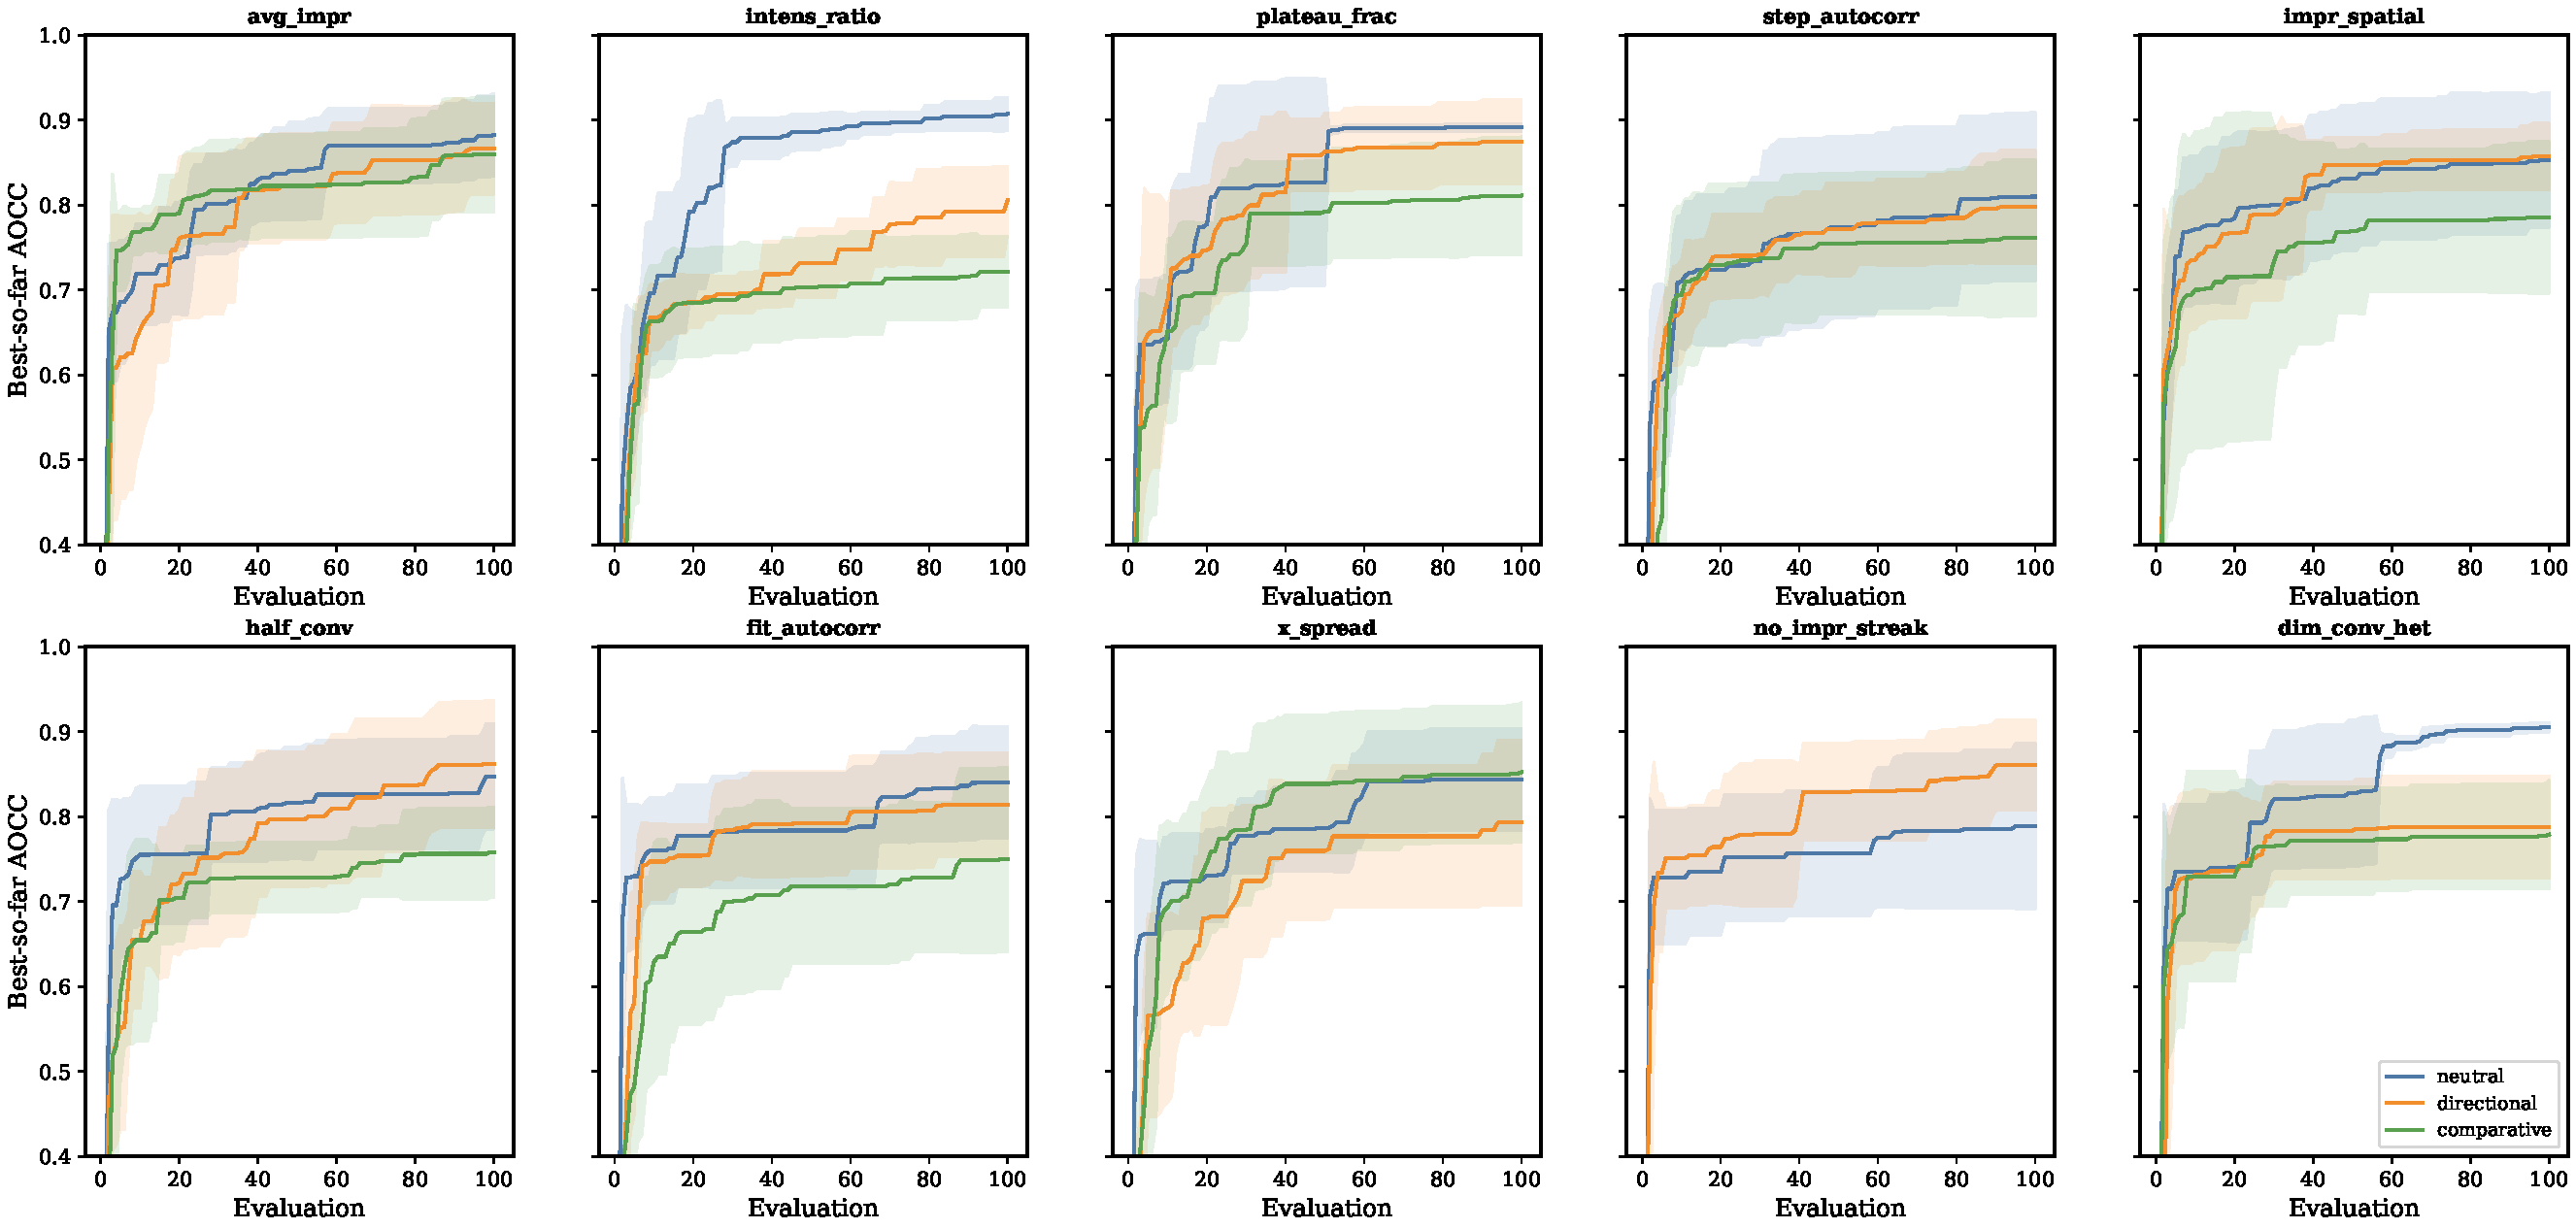
\includegraphics[width=\textwidth]{figures/fig_convergence_by_format.pdf}
  \caption{Best-so-far AOCC over 100 evaluations for each feature, split by feedback format (mean $\pm$ 1 std, 5 seeds). Neutral (blue) typically converges fastest and highest.}
  \label{fig:convergence-by-format}
\end{figure*}

\subsection{Format Ranking}
\label{sec:results-format-ordering}

\Cref{fig:condition-ranking} ranks all 29 conditions by mean best AOCC alongside the vanilla baseline. The top four conditions are all neutral format, and a clear pattern emerges. Neutral conditions cluster at the top, directional in the middle, and comparative at the bottom. To test whether this ordering reflects a genuine difference rather than sampling noise, we apply the Kruskal--Wallis test~\cite{kruskal1952ranks}, a non-parametric alternative to one-way ANOVA that compares the rank distributions of independent groups without assuming normality. The test treats the per-(format, feature) mean AOCCs as independent samples within each format, ignoring the fact that the same feature set appears across formats. A paired Friedman test would be more rigorous, but is complicated by comparative's missing feature. The test confirms a significant difference among formats ($H = 11.5$, $p = 0.003$), with neutral achieving a mean AOCC of $0.855$, directional $0.827$, and comparative $0.784$. The AOCC columns in \cref{tab:steering-detail} show this pattern per feature, with the best format highlighted in bold. Neutral produces the best AOCC for 6 of 10 features, directional for 3, and comparative for just 1. Neutral conditions also have the highest failure rate at $3.5\%$ compared to $2.6\%$ for directional and $1.5\%$ for comparative.

Some behavioural features clearly reduce performance regardless of feedback format. In particular \texttt{step\_size\_autocorrelation}, where even the best format (neutral) achieves only $0.810$. Comparative feedback leads to a reduction in performance relative to neutral for 8 of 9 features, with \texttt{x\_spread\_early} ($+0.008$) being the sole exception. Directional feedback shows more variance. For 6 features it stays within $0.02$ of neutral or beats it outright, while for other 4 it produces drops of $-0.026$ to $-0.117$.

\subsection{Statistical Significance}
\label{sec:results-significance}

Six conditions exceed the vanilla baseline AOCC of $0.862$, four neutral (\texttt{intensification\_ratio}, \texttt{dim\_conv\_heterogeneity}, \texttt{plateau\_fraction}, \texttt{avg\_improvement}) and two directional (\texttt{plateau\_fraction}, \texttt{avg\_improvement}), with \texttt{neutral-intensification\_ratio} at $0.907 \pm 0.021$ performing the best. None of these reach statistical significance against vanilla, and the failure can be attributed to the low number of seeds per condition. With only 5 seeds per group, the Mann--Whitney $U$ test (the two-group form of the Kruskal--Wallis test used above) has limited resolution. There are $\tfrac{10!}{(5!)^2} = 252$ possible ways to interleave the two groups' ranks, so the smallest two-tailed p-value the test can ever produce is $2/252 \approx 0.008$. That minimum is reached only when the two distributions are completely separated, meaning every value in one group exceeds every value in the other. The expected min and max of $n = 5$ samples from a normal distribution sit about $\pm 1.16\,\sigma$ from the mean,\footnote{$1.16 \approx E[X_{(5:5)}]$, the expected value of the largest order statistic in a sample of five standard-normal draws; Blom's approximation $\Phi^{-1}((n - 3/8)/(n + 1/4))$ gives $1.18$ for $n=5$, close to the tabulated value $1.163$.} so separation between vanilla (seed-to-seed AOCC std $\sigma_v = 0.108$) and the best performing condition \texttt{neutral-intensification\_ratio} ($\sigma_b = 0.021$) requires a mean gap exceeding roughly $1.16\,(\sigma_v + \sigma_b) \approx 0.15$. The observed $+0.045$ gap is well below this threshold and the two distributions overlap substantially, so the test cannot rule out chance even though the direction is consistent. Doubling to 10 seeds per condition, as in the Stage~4 setup, raises the number of rank interleavings to $\tfrac{20!}{(10!)^2} = 184{,}756$ and shrinks the minimum detectable effect size by roughly $1/\sqrt{2}$, bringing gaps near the observed $+0.045$ within reach. The seed budget itself was constrained by Gemini API costs. The 29-condition feature$\times$format sweep at 100 candidates per seed already amounts to $14{,}500$ LLaMEA iterations, and doubling to 10 seeds would have cost $29{,}000$ iterations, larger than the entire Stage~4 budget reserved for the head-to-head comparison.

When comparing the three feedback formats against each other for a single behavioural feature, two features do reach statistical significance. With three groups of $n = 5$, the Kruskal--Wallis test has $\tfrac{15!}{(5!)^3} = 756{,}756$ distinct rank assignments and the achievable minimum p-value drops by several orders of magnitude. For \texttt{intensification\_ratio}, neutral ($0.907$) outperforms directional ($0.806$) and comparative ($0.721$) with complete pairwise separation across seeds (Cliff's $d = 1.0$ for every pairwise comparison, Kruskal--Wallis $p = 0.002$). The same holds for \texttt{dim\_conv\_heterogeneity}, where neutral ($0.905$) outperforms directional ($0.788$) and comparative ($0.779$) with no overlap between neutral and either prescriptive format ($d = 1.0$ pairwise, $p = 0.009$).

\subsection{Convergence Dynamics}
\label{sec:results-convergence}

\begin{table*}[t]
\centering
\caption{Feature--AOCC relationship shift from Stage~1 (all models, $n{=}3{,}086$) to Stage~3 (Gemini Flash only, $n{=}14{,}127$). Tier columns show median feature values for bottom-25\% and top-10\% algorithms by AOCC in each stage.}
\label{tab:correlation-shift}
\footnotesize
\begin{tabular}{@{}l|rrrr|rrrr|l@{}}
\toprule
& \multicolumn{4}{c|}{\textbf{Stage 1 (all models)}} & \multicolumn{4}{c|}{\textbf{Stage 3 (Gemini Flash)}} & \\
\textbf{Feature} & \boldmath{$\rho$} & \textbf{Bot25} & \textbf{Top10} & \textbf{Gap} & \boldmath{$\rho$} & \textbf{Bot25} & \textbf{Top10} & \textbf{Gap} & \textbf{Dir.} \\
\midrule
avg\_impr       & $-$.782 & 1.752 & 0.093 & 1.659 & $-$.184 & 0.136 & 0.078 & 0.059 & same \\
intens\_ratio   & $+$.725 & 0.000 & 0.879 & 0.879 & $+$.475 & 0.714 & 0.873 & 0.160 & same \\
plateau\_frac   & $+$.689 & 0.000 & 0.597 & 0.597 & $+$.578 & 0.183 & 0.597 & 0.414 & same \\
step\_autocorr  & $+$.764 & 0.130 & 0.910 & 0.780 & $+$.468 & 0.822 & 0.903 & 0.082 & same \\
impr\_spatial   & $+$.757 & 0.087 & 0.682 & 0.595 & $+$.446 & 0.615 & 0.689 & 0.073 & same \\
half\_conv      & $-$.611 & 0.010 & 0.001 & 0.009 & $-$.640 & 0.003 & 0.001 & 0.002 & same \\
fit\_autocorr   & $+$.650 & 0.003 & 0.766 & 0.764 & $+$.138 & 0.720 & 0.738 & 0.018 & same \\
x\_spread       & $-$.570 & 2.889 & 0.621 & 2.268 & $-$.410 & 1.608 & 0.578 & 1.030 & same \\
longest\_str    & $-$.427 & 6282  & 5543  & 739   & $+$.495 & 1499  & 6018  & 4520  & \textbf{flip} \\
dim\_conv\_het  & $+$.424 & 0.001 & 0.081 & 0.080 & $+$.167 & 0.049 & 0.089 & 0.040 & same \\
\bottomrule
\end{tabular}
\\[0.3em]
{\scriptsize Bot25/Top10 = median feature value among bottom-25\%/top-10\% algorithms by AOCC. Gap = $|$Top10 $-$ Bot25$|$. Dir. = whether correlation direction is preserved.}
\end{table*}

\Cref{fig:convergence-by-format} shows the best-so-far convergence curves for each feature, split by format. The two features with the strongest format effects, \texttt{intensification\_ratio} and \texttt{dim\_conv\_heterogeneity} (the same pair that reach within-feature statistical significance above), show a clear separation early in the run that widens throughout. The features where directional performs well (\texttt{half\_convergence\_time}, \texttt{longest\_streak}) show the formats tracking closely, consistent with the small AOCC deltas reported above. For features like \texttt{average\_improvement}, all three formats converge to similar levels with high variance, showing that this feature does not strongly differentiate performance regardless of how feedback is framed.

\subsection{Behavioural Drift Between Stages}
\label{sec:results-drift}

To validate whether the directional advice itself remains correct in the Stage~3 context, we recompute Spearman correlations between each feature and AOCC on the Stage~3 dataset (\cref{tab:correlation-shift}). Since Stage~3 uses only Gemini~3 Flash, the mean AOCC is higher ($0.646$ vs $0.484$ in Stage~1) and the performance range is narrower. Despite this, 9 of 10 features maintain the same correlation direction, confirming that directional advice is empirically sound.

The correlation magnitudes tell a more nuanced story. Most features weaken substantially, with \texttt{avg\_improvement} showing the most dramatic drop from $\rho = -0.782$ (the strongest correlation in Stage~1) to just $-0.184$ in Stage~3. Only one feature, \texttt{half\_convergence\_time}, strengthens its correlation in the same direction ($-0.611$ to $-0.640$). \texttt{longest\_no\_improvement\_streak} ($-0.427$ to $+0.495$) increases in magnitude but reverses sign, consistent with the non-monotonic relationship that motivated its exclusion from comparative feedback. The reversal points to a broader observation about the pipeline rather than a flaw isolated to this one feature. Everything upstream of Stage~3, both the feature selection in \cref{sec:results-features} and the directional/comparative reference values, was derived from the Stage~1 dataset spanning all 10 models. The 10 features carried forward were chosen because they predicted AOCC across that heterogeneous population, and the prescriptive advice attached to each was calibrated against the same data. When Stage~3 deploys only Gemini~3 Flash, features whose Stage~1 signal was driven mostly by the weaker models retain less predictive power for Flash specifically, and the steering advice inherits some of that mismatch. \texttt{longest\_no\_improvement\_streak} is the most extreme case, but the broader magnitude shrinkage in \cref{tab:correlation-shift} is consistent with a milder version of the same effect operating across many features. The Stage~1 reference remains a reasonable starting point given the cost of running a fresh model-specific screen, but the results suggest that target-model calibration of both feature selection and prescriptive advice would tighten the signal that prescriptive feedback attempts to convey.

\subsection{Behaviour Steering}
\label{sec:results-decoupling}

\begin{figure*}[!t]
  \centering
  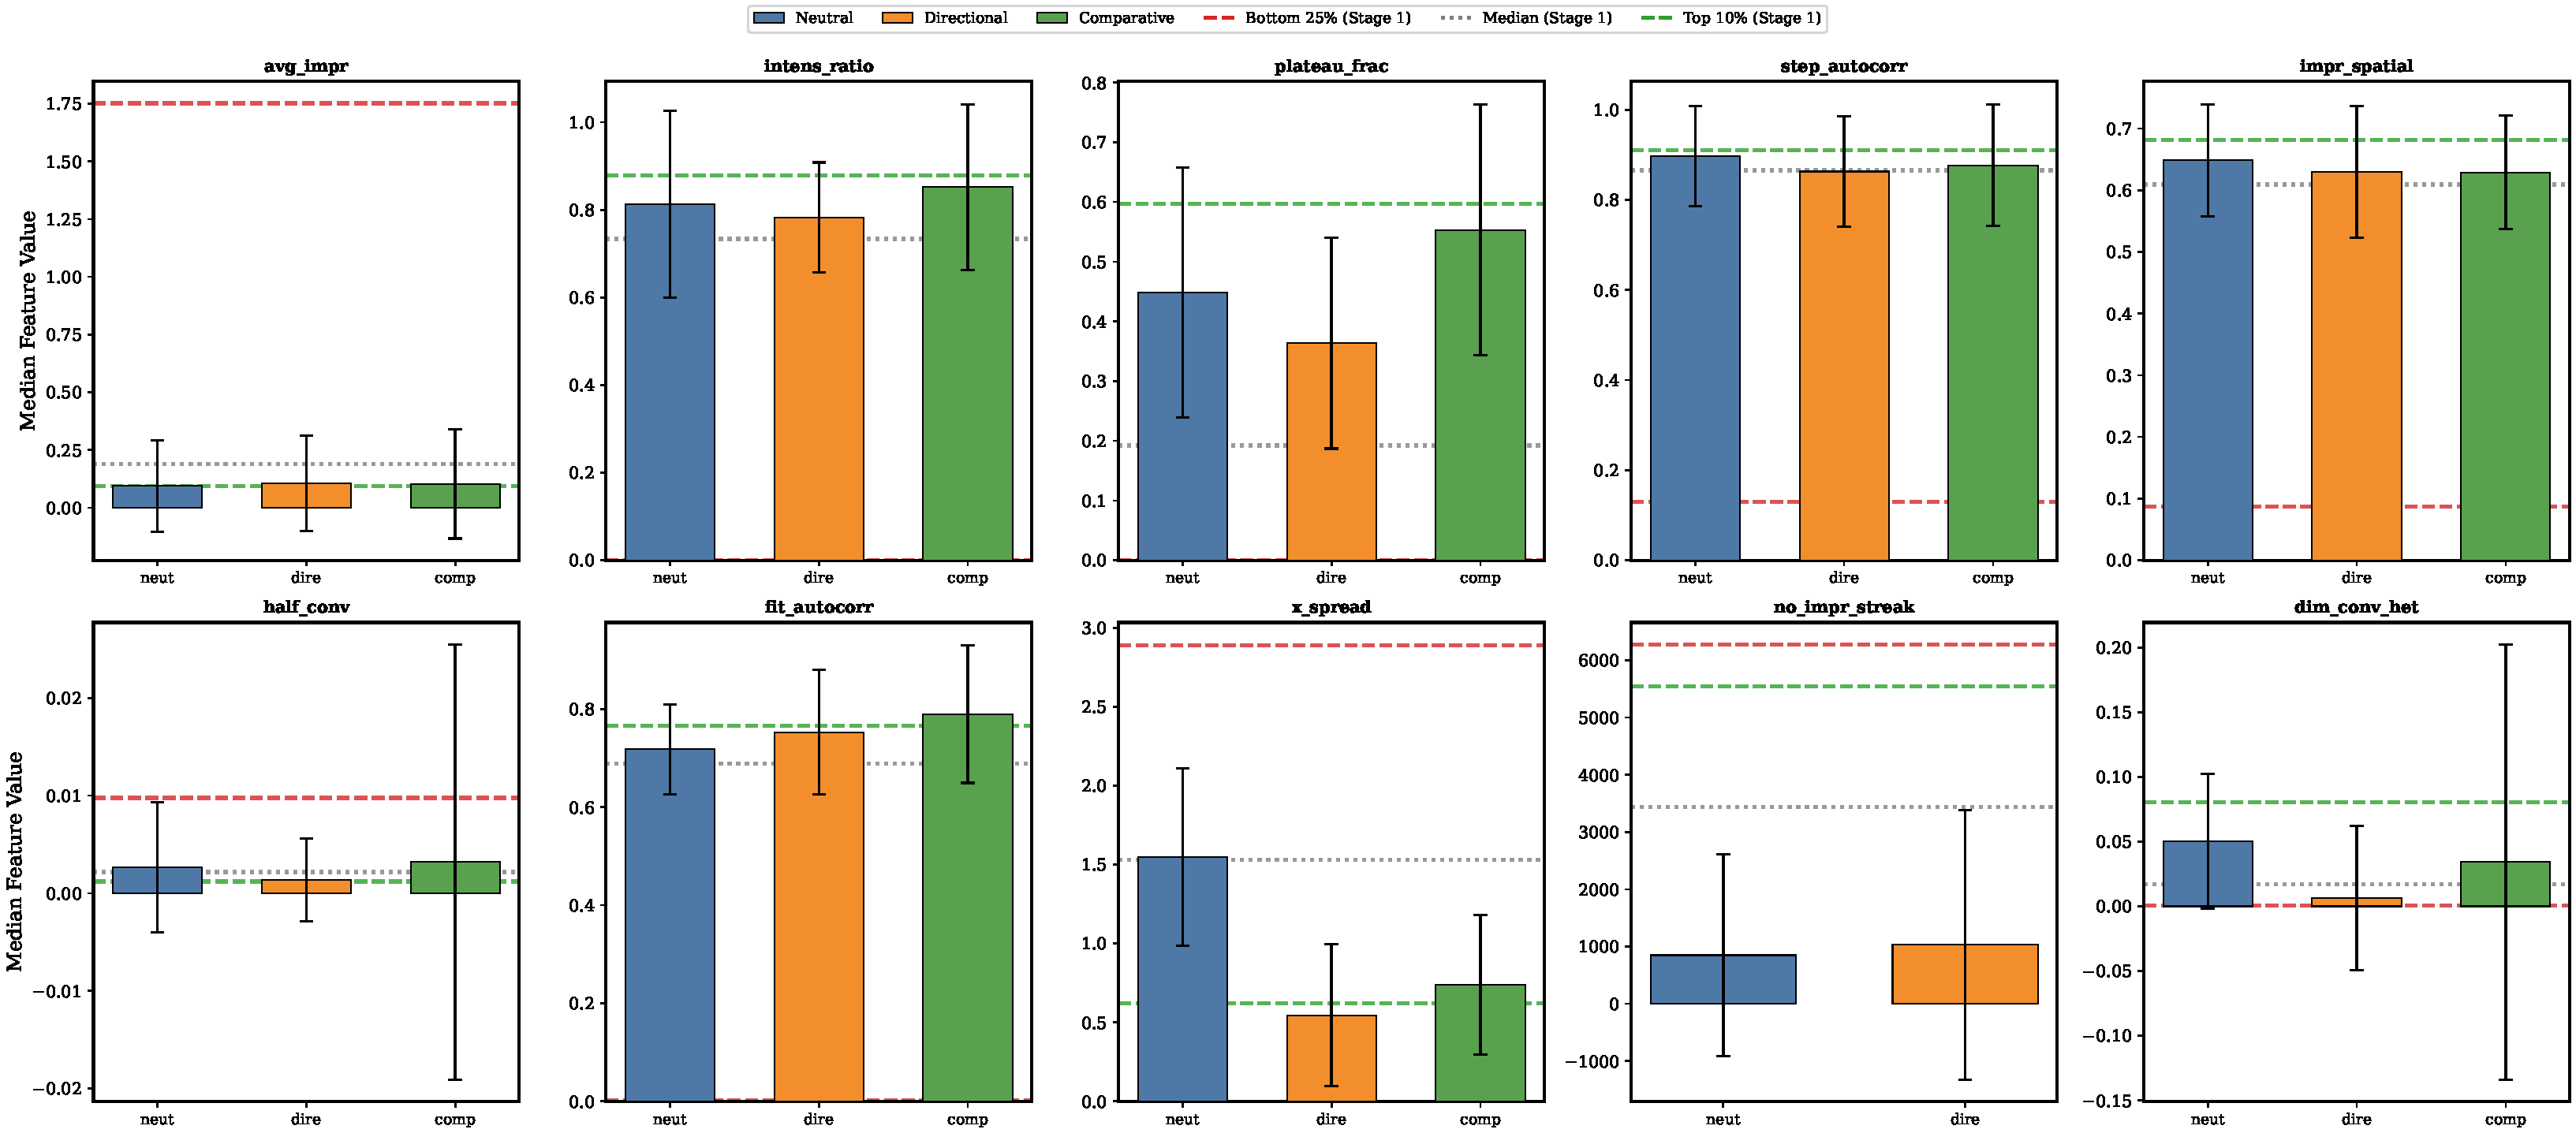
\includegraphics[width=\textwidth]{figures/fig_guided_medians.pdf}
  \caption{Median behavioural feature value by feedback format (bars) compared against Stage~1 AOCC performance tiers (dashed lines): bottom-25\% (red), median (grey), and top-10\% (green). Reference values are computed from all Stage~1 candidates, independent of the feedback experiments.}
  \label{fig:guided-medians}
\end{figure*}

\Cref{tab:steering-detail} shows the median behavioural feature value produced by each format alongside the AOCC, and whether prescriptive feedback steered the feature in the advised direction relative to neutral. \Cref{fig:guided-medians} visualises these values against the Stage~1 AOCC performance tiers.

Across all features, directional feedback steers correctly for 3 of 10 cases and comparative for 4 of 9, giving an overall accuracy of 37\%. Two features (\texttt{fitness\_autocorrelation} and \texttt{x\_spread\_early}) are steered in the correct direction by both guidance formats. Yet for both of these features, correct steering does not translate into better AOCC. For \texttt{x\_spread\_early}, directional feedback correctly reduces the median spread from $1.55$ to $0.55$, well past the top-10\% reference of $0.621$, yet AOCC drops from neutral's $0.844$ to $0.793$. The same pattern appears for \texttt{fitness\_autocorrelation}, where both prescriptive formats increase the value as advised but achieve lower AOCC than neutral. This suggests that pushing a single behavioural value toward its top-tier reference is not, on its own, enough to produce a better algorithm. Strong algorithms are characterised by a combination of feature values, and moving one feature into its high-performing range while leaving the others unconstrained can place a candidate in a region of behaviour space that no actual top-tier algorithm occupies. Comparative feedback compounds this by depending not only on the direction but on the specific reference values it normalises against, which can themselves shift between stages.

\Cref{tab:correlation-shift} shows that the top-10\% reference values stay relatively stable between stages, while the bottom-25\% values shift dramatically. The top-10\% in Stage~1 was already populated mostly by Gemini Flash and Pro candidates, so narrowing to Gemini Flash alone in Stage~3 changes its values very little. The bottom-25\% in Stage~1, by contrast, was populated mostly by the weaker open-weight models, whereas Stage~3's bottom is still produced by Gemini Flash, which is a much stronger generator. For instance, the bottom-25\% of \texttt{step\_size\_autocorrelation} rises from $0.130$ to $0.822$, \texttt{fitness\_autocorrelation} from $0.003$ to $0.720$, and \texttt{intensification\_ratio} from $0.000$ to $0.714$, while their top-10\% values move by less than $0.01$. The gap between the two tiers, which determines the normalisation scale for comparative feedback, therefore collapses by an order of magnitude for several features (e.g., \texttt{fitness\_autocorrelation} from $0.764$ to $0.018$, \texttt{step\_size\_autocorrelation} from $0.780$ to $0.082$, and \texttt{avg\_improvement} from $1.659$ to $0.059$). The distance signals comparative feedback sends become small relative to the actual feature dispersion in Stage~3, blunting their steering effect.

\subsection{Code Complexity}
\label{sec:results-ast}

\begin{table*}[!t]
\centering
\caption{Structural metrics for the $14{,}127$ valid Stage~3 algorithms, parsed via Python's \texttt{ast} module. Columns are grouped into per-format mean $\pm$ std (N = neutral, D = directional, C = comparative; per-format $n \approx 4{,}700$), between-format tests (Kruskal--Wallis $p$ across the three formats and three pairwise Cliff's $d$ effect sizes), and the Spearman rank correlation between the metric and AOCC together with its $p$-value. Rows are sorted by $d_{N\!-\!C}$ descending.}
\label{tab:ast-complexity}
\footnotesize
\setlength{\tabcolsep}{3pt}
\begin{tabular}{@{}l|rrr|rrrr|rr@{}}
\toprule
& \multicolumn{3}{c|}{\textbf{Mean by format}} & \multicolumn{4}{c|}{\textbf{Between-format tests}} & \multicolumn{2}{c}{\textbf{AOCC correlation}} \\
\cmidrule(lr){2-4} \cmidrule(lr){5-8} \cmidrule(lr){9-10}
\textbf{Metric} & \textbf{N} & \textbf{D} & \textbf{C} & \boldmath{$p_{\text{KW}}$} & \boldmath{$d_{N\!-\!C}$} & \boldmath{$d_{N\!-\!D}$} & \boldmath{$d_{D\!-\!C}$} & \boldmath{$p_{\rho}$} & \boldmath{$\rho_{\text{AOCC}}$} \\
\midrule
Total AST nodes                     & 1404$\pm$401   & 1262$\pm$383   & 1145$\pm$409  & $2.4\!\times\!10^{-229}$ & +0.38 & +0.19 & +0.21 & $<\!10^{-300}$ & +0.48 \\
NumPy calls                         & 26.6$\pm$11.2  & 23.4$\pm$10.0  & 19.5$\pm$9.5  & $2.3\!\times\!10^{-223}$ & +0.38 & +0.15 & +0.24 & $<\!10^{-300}$ & +0.60 \\
Assignments                         & 67.5$\pm$15.9  & 63.3$\pm$16.2  & 58.0$\pm$15.6 & $4.9\!\times\!10^{-192}$ & +0.35 & +0.15 & +0.21 & $<\!10^{-300}$ & +0.40 \\
\texttt{try}/\texttt{except} blocks & 0.5$\pm$0.6    & 0.3$\pm$0.6    & 0.2$\pm$0.4   & $5.1\!\times\!10^{-200}$ & +0.28 & +0.20 & +0.08 & $<\!10^{-300}$ & +0.48 \\
\texttt{return} stmts               & 2.3$\pm$1.2    & 2.0$\pm$1.2    & 1.9$\pm$1.3   & $2.2\!\times\!10^{-123}$ & +0.26 & +0.16 & +0.12 & $7.0\!\times\!10^{-4}$ & +0.03 \\
\texttt{while} loops                & 3.0$\pm$1.4    & 2.8$\pm$1.3    & 2.4$\pm$1.2   & $2.5\!\times\!10^{-90}$  & +0.22 & +0.06 & +0.17 & $2.8\!\times\!10^{-73}$ & $-$0.15 \\
\texttt{for} loops                  & 2.4$\pm$1.3    & 2.2$\pm$1.4    & 2.0$\pm$1.5   & $3.8\!\times\!10^{-63}$  & +0.20 & +0.08 & +0.11 & $1.3\!\times\!10^{-12}$ & +0.06 \\
Max loop depth                      & 3.0$\pm$0.6    & 2.9$\pm$0.7    & 2.7$\pm$0.7   & $2.5\!\times\!10^{-81}$  & +0.19 & +0.03 & +0.15 & $2.8\!\times\!10^{-86}$ & +0.16 \\
Numeric constants                   & 70.2$\pm$32.7  & 63.1$\pm$26.6  & 58.6$\pm$24.1 & $1.3\!\times\!10^{-36}$  & +0.15 & +0.08 & +0.09 & $<\!10^{-300}$ & +0.66 \\
Function definitions                & 2.6$\pm$0.8    & 2.4$\pm$0.8    & 2.4$\pm$0.8   & $8.0\!\times\!10^{-35}$  & +0.12 & +0.09 & +0.04 & $7.2\!\times\!10^{-172}$ & +0.23 \\
\texttt{if} branches                & 13.6$\pm$4.3   & 13.8$\pm$4.1   & 13.5$\pm$4.6  & $5.0\!\times\!10^{-14}$  & +0.05 & $-$0.05 & +0.09 & $3.8\!\times\!10^{-81}$ & +0.16 \\
Augmented assigns                   & 5.9$\pm$3.8    & 6.4$\pm$3.3    & 6.6$\pm$3.1   & $1.7\!\times\!10^{-29}$  & $-$0.13 & $-$0.09 & $-$0.05 & $<\!10^{-300}$ & +0.47 \\
\bottomrule
\end{tabular}
\\[0.3em]
{\scriptsize $p_{\text{KW}}$ is the Kruskal--Wallis omnibus test that the three format distributions differ at all. Cliff's $d \in [-1, +1]$ measures pairwise rank dominance: $|d| < 0.147$ negligible, $0.147$--$0.33$ small, $0.33$--$0.474$ medium, $\geq 0.474$ large. $\rho_{\text{AOCC}}$ is the Spearman rank correlation between the metric and AOCC across all $14{,}127$ algorithms; $p_{\rho}$ is its two-sided significance. Values reported as $<\!10^{-300}$ underflow scipy's floating-point precision. NumPy calls = \texttt{ast.Call} nodes whose target is a method on the \texttt{np} namespace; numeric constants count integer and float literals.}
\end{table*}

We measure structural complexity by parsing every valid Stage~3 algorithm with Python's \texttt{ast} module and extracting twelve metrics covering raw size, arithmetic content, and control-flow structure (\cref{tab:ast-complexity}). We find that neutral feedback produces more complex code than other conditions. We test for between-format differences using Kruskal--Wallis on each metric. At $\sim4{,}700$ algorithms per format, the test rejects the null at $p < 10^{-13}$ on every row, so effect sizes rather than significance carry the comparison. The largest pairwise gap on each of the formats is between neutral and comparative. Cliff's $d$ ($d_{N\!-\!C}$) is at least $+0.20$ (small effect or larger) on six of twelve metrics: total AST nodes, NumPy calls, assignments, \texttt{try}/\texttt{except} blocks, \texttt{return} statements, and \texttt{while} loops. Directional sits between the other two formats, with $d_{N\!-\!D}$ and $d_{D\!-\!C}$ both smaller and of the same sign as $d_{N\!-\!C}$ with the exception of the \texttt{if} branches condition. This reproduces the format ordering seen in the AOCC ranking of \cref{sec:results-format-ordering}.

We test the metric--AOCC association with Spearman rank correlation across the full set. All twelve correlations are statistically significant. Features that measure code complexity such as total AST nodes ($\rho_{\text{AOCC}} = +0.48$), NumPy calls ($+0.60$), and numeric constants ($+0.66$) show the strongest correlations with AOCC. Together with the per-format gap above, this offers a candidate explanation for the format ranking in \cref{sec:results-format-ordering}. Neutral pushes the LLM toward more elaborate code on the same axes that correlate with stronger optimisation performance.

% ===========================================================================
\section{Full-Benchmark Comparison}
\label{sec:results-stage4}

The Stage~4 dataset contains $16{,}538$ valid candidates produced by Gemini~3 Flash across four feedback conditions (vanilla, neutral-behavioural, SAGE, combined) at 500 candidates per seed and 10 seeds per condition, evaluated on 20 disjoint MA-BBOB functions with five instance seeds each. This section reports the head-to-head comparison: aggregate condition performance, per-instance robustness, failure-rate dynamics, behavioural steering at scale, and the identity of the best-found algorithm in each condition.

\begin{figure}[t]
  \centering
  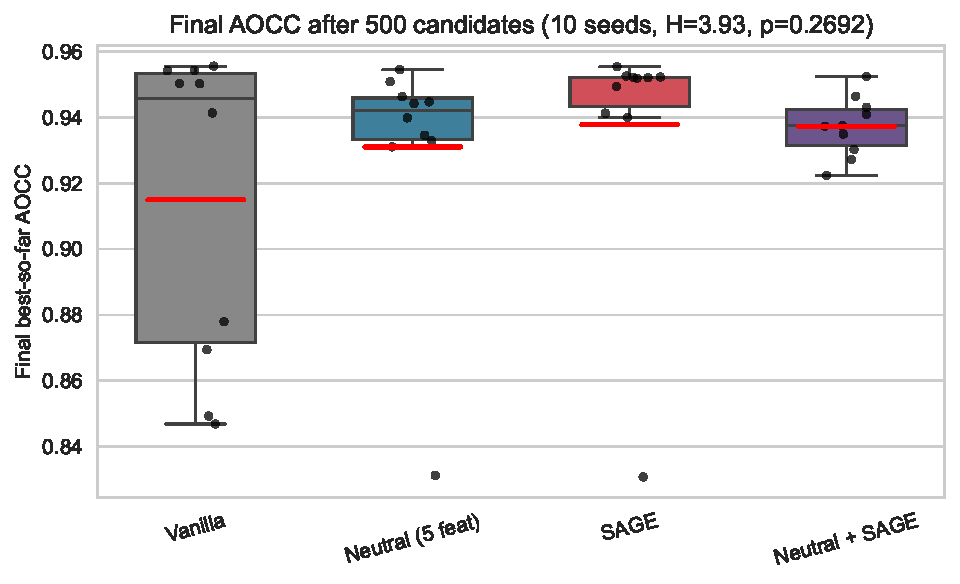
\includegraphics[width=\columnwidth]{figures/fig_phase4_final_aocc.pdf}
  \caption{Final best-so-far AOCC after 500 candidates, 10 seeds per condition. Box shows quartiles, whisker shows 1.5$\times$IQR, individual seeds plotted as black dots. Red bar marks the per-condition mean.}
  \label{fig:phase4-final-aocc}
\end{figure}

\begin{figure}[t]
  \centering
  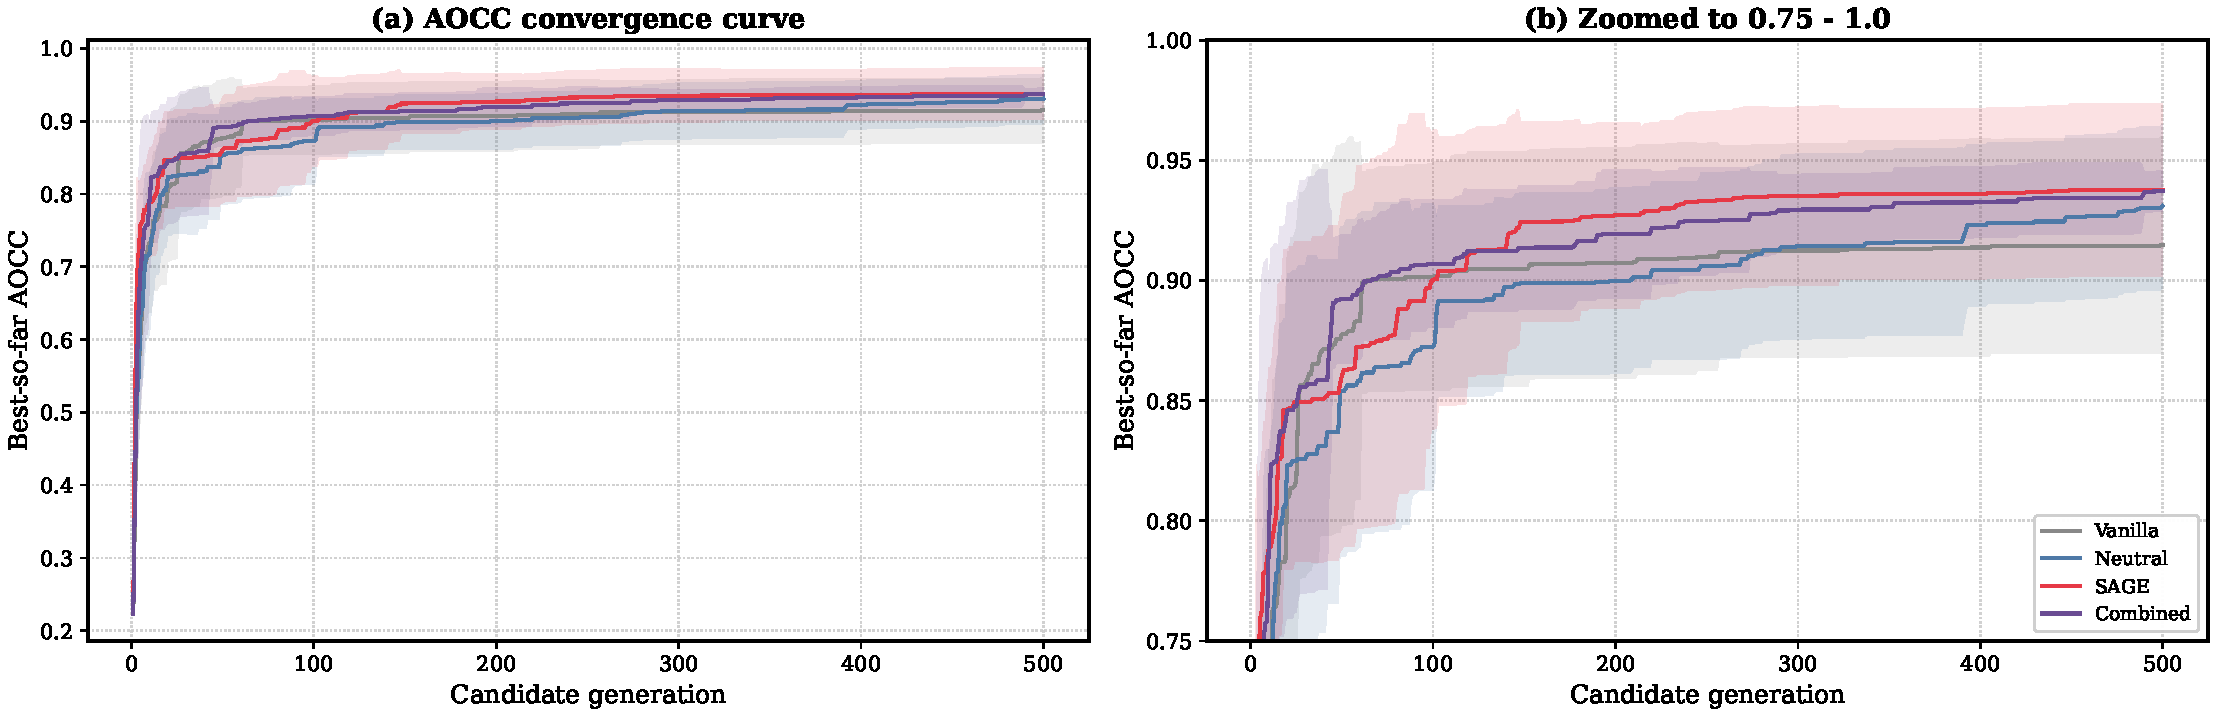
\includegraphics[width=\columnwidth]{figures/fig_phase4_convergence.pdf}
  \caption{Best-so-far AOCC across the 500-candidate budget, mean across 10 seeds with 95\% bootstrap CI ribbon ($n_{\text{boot}}{=}1{,}000$).}
  \label{fig:phase4-convergence}
\end{figure}

% ---------------------------------------------------------------------------
\subsection{Aggregate Condition Performance}
\label{sec:results-stage4-agg}

\Cref{fig:phase4-final-aocc} shows the final best-so-far AOCC distribution across 10 seeds per condition. The condition means rank vanilla ($0.915 \pm 0.048$) below neutral ($0.931 \pm 0.036$), SAGE ($0.938 \pm 0.038$), and combined ($0.937 \pm 0.009$). All three feedback-augmented conditions produce a higher mean than vanilla, and the spread shrinks substantially under combined, whose seed-to-seed standard deviation is roughly five times smaller than vanilla's. \Cref{fig:phase4-convergence} visualises this through the convergence trajectories with a 95\% bootstrap CI ribbon. The four conditions begin overlapping over the first $\sim$50 candidates, then separate from generation 100 onward, with the vanilla curve broadening visibly compared to the three feedback-augmented conditions.

The Kruskal--Wallis test across the four conditions returns $H = 3.93,\, p = 0.27$, so the means do not differ at $p < 0.05$. The minimum two-tailed $p$-value attainable from a four-group Kruskal--Wallis with $n = 10$ per group is roughly $10^{-3}$, but only when all four distributions are completely separated. With $\Delta\text{AOCC} \le 0.023$ between the worst-performing (vanilla) and best-performing (SAGE) condition means and seed-level standard deviations of $0.04$--$0.05$, the per-seed distributions overlap and the test cannot reject the null. Holm-corrected pairwise Mann--Whitney comparisons return $p \ge 0.23$ for every pair, with the largest unadjusted gap (sage vs combined, $p_{\text{raw}} = 0.038$) inflated to $p_{\text{Holm}} = 0.226$ after correction for six tests. The 10-seed budget improves resolution over Stage~3's 5-seed setup, but the observed condition means stay within the Stage~3 noise floor identified in \cref{sec:results-significance}.

\begin{figure}[t]
  \centering
  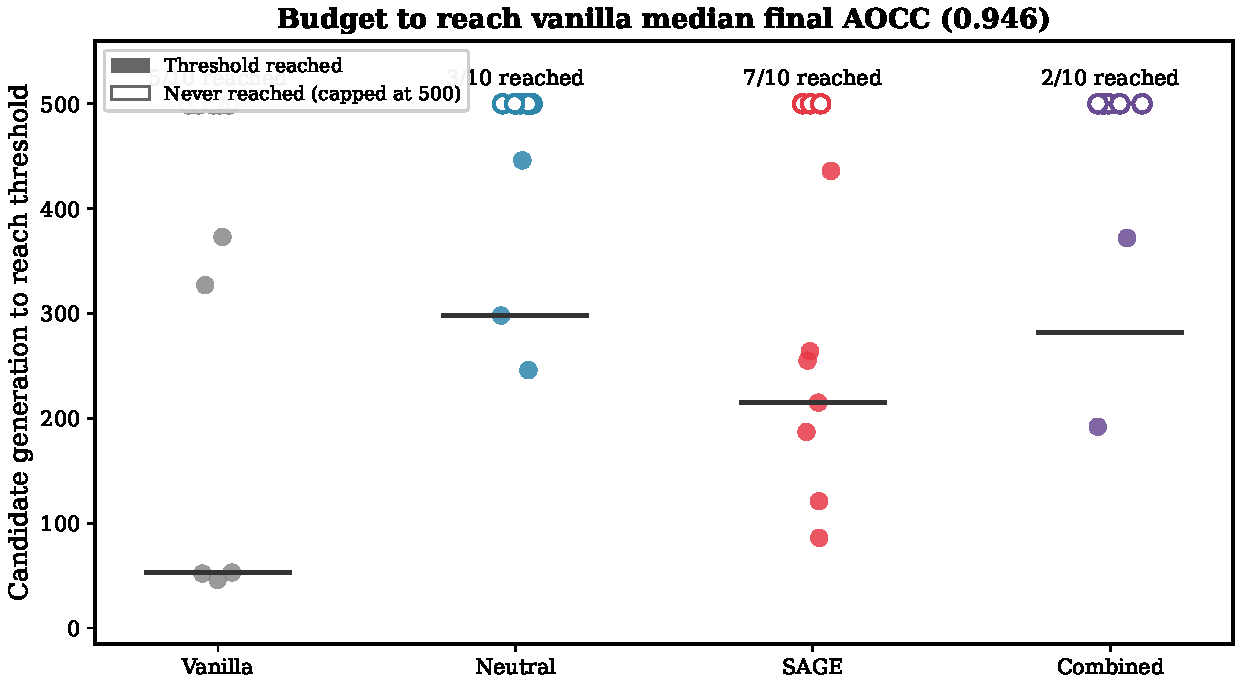
\includegraphics[width=\columnwidth]{figures/fig_phase4_budget_threshold.pdf}
  \caption{Number of generations needed for each seed to reach the vanilla median final AOCC threshold (0.946). Open markers indicate seeds that never reached the threshold within 500 generations.}
  \label{fig:phase4-budget}
\end{figure}

A second view of the comparison is the budget-to-threshold metric, which records how many generations each seed needed to reach the vanilla median final AOCC of $0.946$ (\cref{fig:phase4-budget}). The fraction of seeds that ever reach the threshold differs sharply between conditions: SAGE reaches it in $7$ of $10$ seeds, vanilla in $5$ of $10$, neutral in $3$ of $10$, and combined in $2$ of $10$. SAGE also reaches the threshold most consistently, with a median of $216$ generations and a range of $\pm 115$. Vanilla's median of $54$ is the fastest among reaching seeds but is driven by a few quickly-converging seeds, with the remaining seeds plateauing well below the threshold. Combined's high mean ($0.937$) and low variance ($\sigma = 0.009$) mean its seeds cluster tightly near, but mostly below, the threshold.

% ---------------------------------------------------------------------------
\subsection{Per-Instance Robustness}
\label{sec:results-stage4-perinstance}

\begin{figure*}[t]
  \centering
  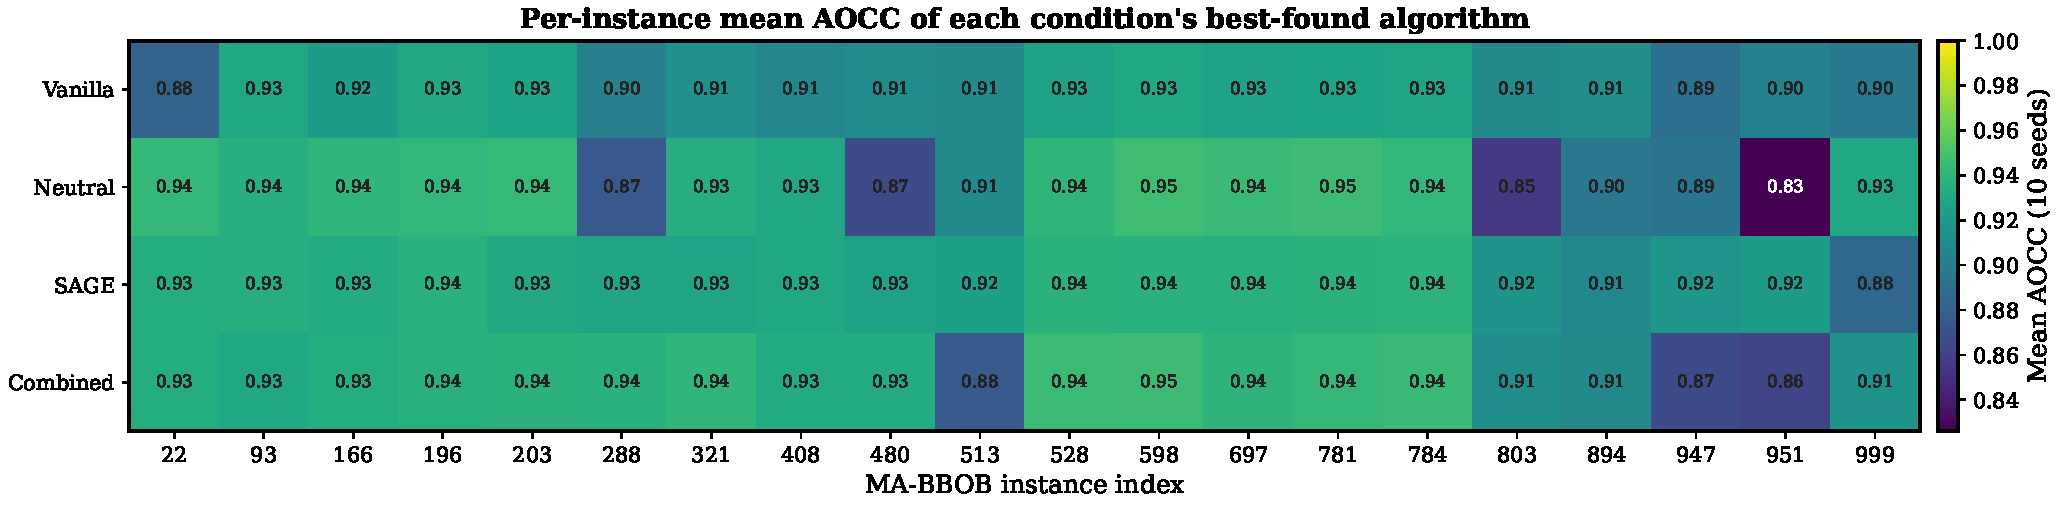
\includegraphics[width=\textwidth]{figures/fig_phase4_per_instance.pdf}
  \caption{Per-instance mean AOCC of each condition's best-found algorithm across the 20 MA-BBOB functions in the Stage~4 set. Each cell averages 10 seeds.}
  \label{fig:phase4-per-instance}
\end{figure*}

\Cref{fig:phase4-per-instance} drills the comparison down to per-instance behaviour. For each (condition, seed) we take the final best-so-far candidate's AOCC on each of the 20 MA-BBOB functions and average across the 10 seeds. SAGE and combined dominate on most instances with mean per-instance AOCC above $0.93$. Vanilla shows a few instances where a single seed's best-so-far happens to find a strong algorithm, but the across-seed average lags by 0.02--0.05 on instances such as 22, 166, and 528. The hardest instance for every condition is 203, with means clustered around 0.85--0.89. No instance flips the condition ordering. The vanilla condition is never the strongest on any instance averaged across seeds.

% ---------------------------------------------------------------------------
\subsection{Failure-Rate Analysis}
\label{sec:results-stage4-failures}

\begin{figure}[t]
  \centering
  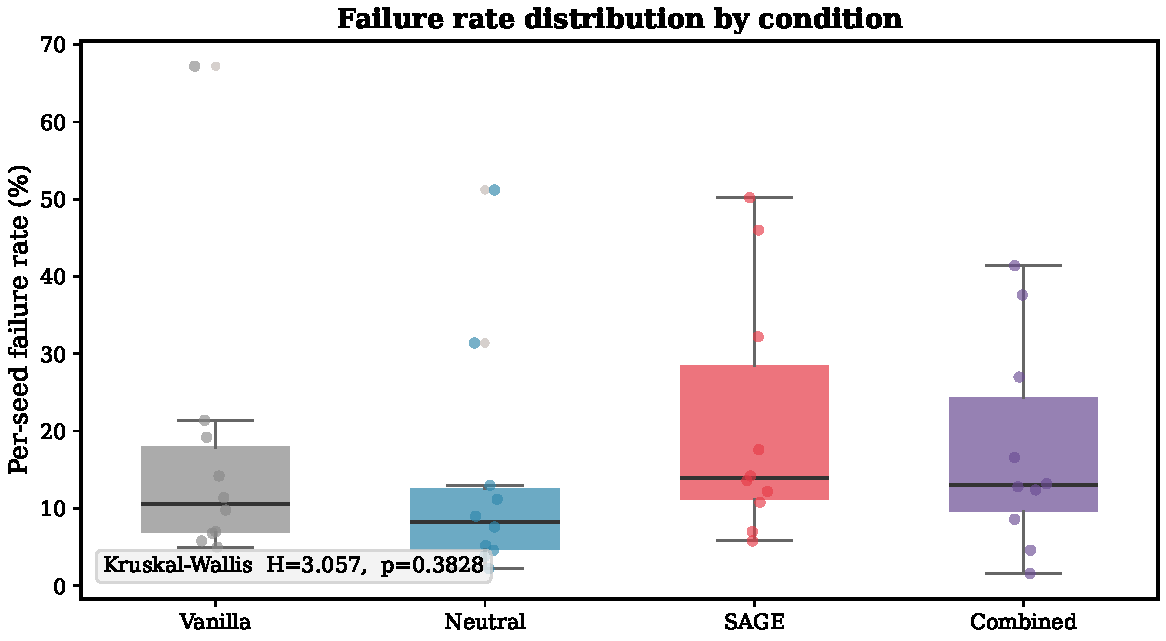
\includegraphics[width=\columnwidth]{figures/fig_phase4_failure_rates.pdf}
  \caption{Per-seed failure rate distribution by condition (10 seeds per condition, 500 candidates per seed).}
  \label{fig:phase4-failures}
\end{figure}

\begin{table}[t]
\centering
\caption{Stage~4 failure-mode breakdown by condition. Each row sums to the total failed-candidate count for that condition and gives per-mode counts and (in parentheses) percentages. \emph{Unclass.\ success} marks failures whose source code passes the BLADE compile-and-smoke pipeline post-hoc; the row totals therefore agree with the recorded failure counts even though those candidates ran cleanly under retry.}
\label{tab:phase4-failure-modes}
\footnotesize
\setlength{\tabcolsep}{4pt}
\begin{tabular}{@{}l|rrrrr|r@{}}
\toprule
\textbf{Cond.} & \textbf{CodeGen} & \textbf{Import} & \textbf{Iface} & \textbf{Runtime} & \textbf{Unclass.} & \textbf{Tot.} \\
\midrule
vanilla   & 9 (1.1)   & 34 (4.1)   & 1 (0.1)   & 710 (84.6) & 85 (10.1) & 839  \\
neutral   & 23 (3.3)  & 26 (3.7)   & 7 (1.0)   & 620 (89.1) & 20 (2.9)  & 696  \\
sage      & 8 (0.8)   & 151 (14.4) & 10 (1.0)  & 867 (82.7) & 12 (1.1)  & 1048 \\
combined  & 16 (1.8)  & 36 (4.1)   & 38 (4.3)  & 770 (87.6) & 19 (2.2)  & 879  \\
\bottomrule
\end{tabular}
\\[0.3em]
{\scriptsize CodeGen = no class produced or syntax error; Import = disallowed package; Iface = \texttt{\_\_init\_\_(budget, dim)} or \texttt{\_\_call\_\_(func)} signature mismatch; Runtime = exception during the post-hoc smoke test on BBOB f11. The \emph{unclass.} column re-runs the candidate through BLADE's compile-and-smoke pipeline; cases where the smoke test now passes are flagged as unclassified, indicating the original failure was instance- or dim-specific in the full MA-BBOB evaluation rather than reproducible at the smoke-test stage.}
\end{table}

The Stage~3 failure analysis identified runtime errors as the dominant mode for capable models. Stage~4 reproduces this. Across the four conditions, vanilla fails on 16.8\% of candidates, neutral on 13.9\%, SAGE on 21.0\%, and combined on 17.6\% (Kruskal--Wallis on per-seed failure rates: $H = 3.06,\, p = 0.38$). SAGE's higher failure rate is consistent with the prior observation that its structural advice pushes the LLM toward more elaborate, error-prone code.

To recover the failure category for each event we replay the candidate's source through the same compile-and-smoke pipeline that BLADE uses at runtime, with a 10-second per-candidate timeout to bound infinite loops. \Cref{tab:phase4-failure-modes} reports the breakdown. Runtime errors dominate every condition (between 82.7\% and 89.1\% of failures). The conditions differ on the lower-frequency modes that reflect feedback-driven habits. SAGE produces 14.4\% import-violation failures, more than three times any other condition, as its complexity-oriented advice repeatedly pulls in libraries beyond the allowed \texttt{numpy}-only environment (e.g., \texttt{scipy.optimize}, \texttt{sklearn}). Combined drives interface mismatches to 4.3\%, four times any other condition, suggesting that bundling behavioural and structural advice occasionally leads the LLM to alter the prescribed \texttt{\_\_init\_\_(budget, dim)} or \texttt{\_\_call\_\_(func)} signature in ways that break the framework contract. Vanilla stands out for its high \emph{unclassified-success} rate of 10.1\%, where the smoke replay now compiles and runs but the original phase recorded a failure. These cases correspond to candidates whose error appears in the larger MA-BBOB evaluation (a specific function or instance triggers a numerical edge case) rather than at the BBOB-f11 smoke stage.

\begin{figure}[t]
  \centering
  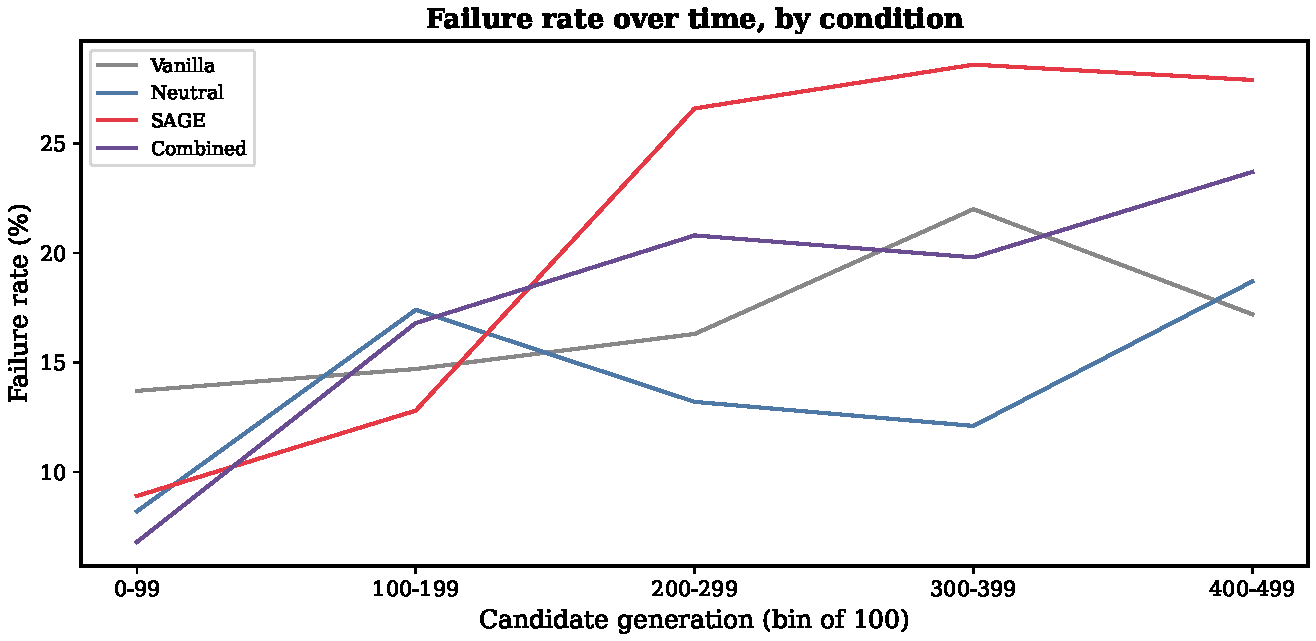
\includegraphics[width=\columnwidth]{figures/fig_phase4_failure_by_gen.pdf}
  \caption{Failure rate by 100-candidate generation bin, per condition. Failure brittleness compounds over time most strongly under SAGE.}
  \label{fig:phase4-failure-bygen}
\end{figure}

\Cref{fig:phase4-failure-bygen} bins the same failures by generation. SAGE's failure rate climbs from 8.9\% in the first 100 generations to 27.9\% in generations 400--499, more than tripling. Combined climbs more gently from 6.8\% to 23.7\%. Vanilla and neutral oscillate between 12\% and 22\% with no clear trend. The compounding pattern under SAGE is consistent with its mechanism: structural advice accumulates archive entries each generation, and as the prompt grows the LLM is increasingly nudged into elaborate code paths that fail to satisfy the simulation environment.

% ---------------------------------------------------------------------------
\subsection{Behavioural Profiles and Steering}
\label{sec:results-stage4-steering}

\begin{figure*}[t]
  \centering
  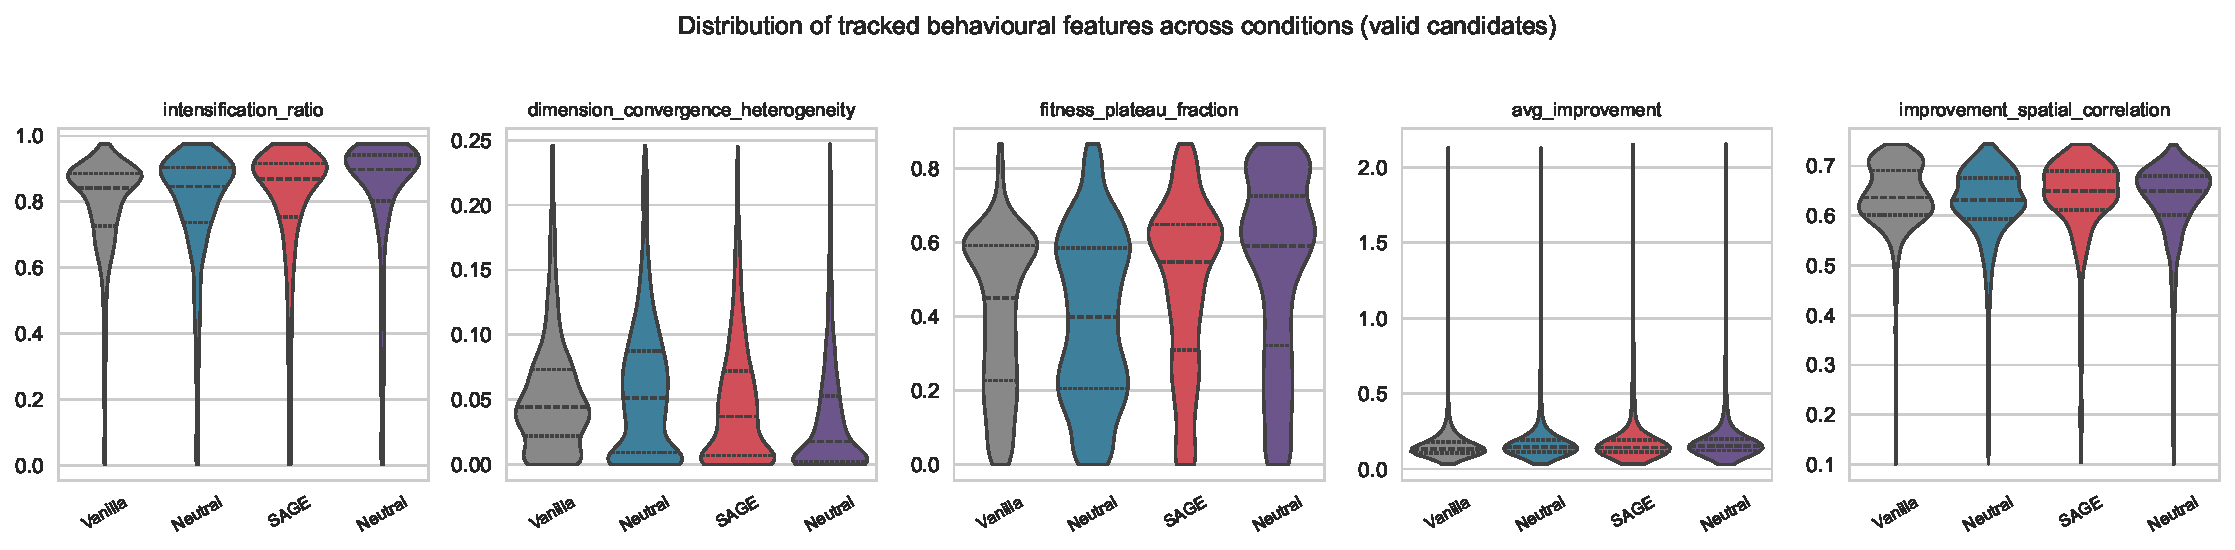
\includegraphics[width=\textwidth]{figures/fig_phase4_behavioural.pdf}
  \caption{Distribution of the five tracked behavioural features across all valid Stage~4 candidates by condition. Each violin spans the full per-condition distribution; black bars mark the median. The five features are those carried forward from Stage~3 (\cref{sec:meth-stage4}).}
  \label{fig:phase4-behavioural}
\end{figure*}

\begin{table}[t]
\centering
\caption{Per-feature behavioural steering rate. Each cell reports the fraction of valid candidates in the listed condition whose feature value lies on the advised side of vanilla's median (Stage~1 advised direction in parentheses). Bold marks rates above 60\%; italicised values below 50\% indicate the condition steers \emph{away} from the advised direction.}
\label{tab:phase4-steering-rates}
\footnotesize
\setlength{\tabcolsep}{4pt}
\begin{tabular}{@{}l|rrr@{}}
\toprule
\textbf{Feature (advised)} & \textbf{Neutral} & \textbf{SAGE} & \textbf{Combined} \\
\midrule
intensification\_ratio ($\uparrow$)  & 51.9             & 58.3             & \textbf{69.3} \\
fitness\_plateau\_fraction ($\uparrow$) & \textit{44.2} & \textbf{62.1}    & \textbf{66.5} \\
impr\_spatial\_correlation ($\uparrow$) & \textit{46.3} & 58.2             & 58.4 \\
dim\_conv\_heterogeneity ($\uparrow$)   & 54.4          & \textit{43.4}    & \textit{30.3} \\
avg\_improvement ($\downarrow$)         & \textit{41.9} & \textit{40.9}    & \textit{34.5} \\
\bottomrule
\end{tabular}
\end{table}

\Cref{fig:phase4-behavioural} shows the distribution of the five tracked behavioural features across all valid candidates, by condition. Combined produces the most concentrated distributions on \texttt{intensification\_ratio} and \texttt{fitness\_plateau\_fraction}, the two features most strongly linked to high AOCC in the Stage~1 analysis. SAGE's distributions track combined closely on these two features, and both lie above neutral and vanilla. \texttt{dim\_conv\_heterogeneity} shows the opposite pattern: combined's distribution is the lowest of the four conditions, despite higher being advised.

To quantify steering directly we compute, for each (feature, condition) pair, the percentage of candidates whose feature value lies on the advised side of vanilla's median. \Cref{tab:phase4-steering-rates} reports the rates. Combined steers strongest on \texttt{intensification\_ratio} ($69.3\%$), \texttt{fitness\_plateau\_fraction} ($66.5\%$), and \texttt{impr\_spatial\_correlation} ($58.4\%$). SAGE achieves comparable rates on those three features without seeing them in its prompt, since SAGE's structural advice is correlated with code patterns that produce intensified, plateau-rich trajectories~\cite{vanStein2026LLaMEASAGE}. Neutral, despite explicitly receiving these features as feedback, lands only slightly above $50\%$ on intensification ($51.9\%$) and \emph{below} $50\%$ on plateau ($44.2\%$) and spatial correlation ($46.3\%$).

Two failures of steering stand out. First, every condition steers in the wrong direction on \texttt{avg\_improvement}. Lower values are advised because they indicate the algorithm has already exhausted easy gains, but combined ($34.5\%$), SAGE ($40.9\%$), and neutral ($41.9\%$) all sit below $50\%$. Second, combined drives \texttt{dim\_conv\_heterogeneity} dramatically away from advised ($30.3\%$, with SAGE at $43.4\%$). Both features had moderate-to-strong correlations with AOCC in Stage~1 but suffered the largest correlation drift to Stage~3 (\cref{tab:correlation-shift}); the Stage~4 steering pattern is consistent with the Stage~3 result that prescriptive advice loses traction when the underlying signal weakens between the calibration and deployment populations. The pattern reinforces the Stage~3 sub-finding that correctly reporting a feature does not guarantee the LLM moves it as advised, especially for features whose signal is weak or non-monotonic in the deployed population.

% ---------------------------------------------------------------------------
\subsection{Best-Found Algorithm Identity}
\label{sec:results-stage4-winners}

\begin{table}[t]
\centering
\caption{Best-found algorithm in each Stage~4 condition (highest final best-so-far AOCC across the 10 seeds). Static code metrics computed on the generated source: lines of code (excluding blanks and comments) and maximum block-nesting depth (counted from indentation).}
\label{tab:phase4-winners}
\footnotesize
\setlength{\tabcolsep}{4pt}
\begin{tabular}{@{}l|llrrr@{}}
\toprule
\textbf{Cond.} & \textbf{Algorithm name} & \textbf{Seed} & \textbf{AOCC} & \textbf{LoC} & \textbf{Nest} \\
\midrule
vanilla  & \texttt{IGA\_CMA}          & 3 & 0.9555 & 106 & 6 \\
neutral  & \texttt{BIPOP\_MA\_CMA\_ES} & 0 & 0.9545 & 115 & 6 \\
sage     & \texttt{CMA\_EES}          & 5 & 0.9554 &  95 & 6 \\
combined & \texttt{OM\_CMA\_EIS}       & 7 & 0.9524 &  95 & 6 \\
\bottomrule
\end{tabular}
\end{table}

\Cref{tab:phase4-winners} reports the best-found algorithm per condition, taken as the candidate with the highest final best-so-far AOCC across the 10 seeds. The four winners span only a $0.0031$ AOCC range, and all four are CMA-ES variants: \texttt{IGA\_CMA}, \texttt{BIPOP\_MA\_CMA\_ES}, \texttt{CMA\_EES}, and \texttt{OM\_CMA\_EIS}, each between 95 and 115 lines of code with maximum nesting depth 6. The full source for all four is reproduced in \cref{app:stage4-winners}. The best-performing algorithm of every condition is therefore a CMA-ES variant, regardless of the feedback string Gemini~3 Flash sees. This is an indication of a model bias: when asked for a high-quality black-box optimiser on MA-BBOB, Gemini snaps to CMA-ES even when the feedback explicitly steers toward different behavioural targets. The bias does not necessarily reflect a flaw, since CMA-ES is genuinely state of the art on this class of benchmark; it does, however, mean that the feedback string does not move the model off this default family.

Reading the four sources confirms the family bias in detail. Every winner reproduces the canonical Hansen tutorial of CMA-ES: log-decreasing recombination weights, the standard learning-rate constants $c_c, c_s, c_1, c_\mu, d_{\text{amps}}, \chi_n$ verbatim, both evolution paths $p_c$ and $p_s$, the Heaviside $h_\sigma$ indicator, the rank-1 + rank-$\mu$ covariance update, and CSA step-size control. None of the winners replaces, simplifies, or fundamentally re-derives this core; each decorates it with two or three heuristic add-ons.

Three add-ons recur. Mirrored sampling --- antithetic $\pm z$ pairs to halve sampling noise on the mean shift --- appears in all four winners. QR-decomposed orthogonal sampling also appears in all four, applied to a randn matrix and rescaled by $\sqrt{n}$ (low-dim-only in \texttt{BIPOP\_MA\_CMA\_ES}). Active CMA with negative rank-$\mu$ weights appears in two: \texttt{IGA\_CMA}, with an aggressive flat $-0.8$ negative coefficient, and \texttt{BIPOP\_MA\_CMA\_ES}, capped at $0.5\,c_\mu$. The conditions diverge on the remaining heuristic interventions:

\begin{itemize}
  \item \texttt{IGA\_CMA} (vanilla) wraps the inner CMA in an IPOP-style restart loop that doubles population size on collapse, layered with a DE-style mean-injection step that overrides $x_{\text{mean}}$ on stagnation and a biased re-initialisation that draws the new mean near the running best with probability $0.3$.
  \item \texttt{BIPOP\_MA\_CMA\_ES} (neutral) scaffolds BIPOP --- alternating between large- and small-population regimes on each restart --- but omits the canonical Hansen 2009 budget accounting that selects the next regime; an unused \texttt{success\_history} list and the absence of any local-search make the ``MA'' (memetic) prefix decorative.
  \item \texttt{CMA\_EES} (SAGE) adds edge-biased radial scaling on the orthogonal samples (a $\text{Beta}(0.5, 0.5)$ mixed into the $\chi$-scale) and modulo-reflective boundary handling that bounces out-of-bounds points back into the interior. Restart is conservative: only on near-total stagnation, and suppressed past $80\%$ of the FE budget.
  \item \texttt{OM\_CMA\_EIS} (combined) injects a momentum term --- an exponential moving average of recent mean-shift directions --- into each sample, biasing offspring along the recent successful trajectory. There is no proper restart, only a $1.1\times$ sigma kick when the within-generation fitness range collapses.
\end{itemize}

Several of the tweaks are also of dubious correctness. The mirrored-and-orthogonalised samples in \texttt{BIPOP\_MA\_CMA\_ES}, \texttt{CMA\_EES}, and \texttt{OM\_CMA\_EIS} break the Gaussian assumption that CSA's expected step-norm $\chi_n$ relies on. Bare \texttt{except} clauses in three of the four winners silently fall back to an identity covariance on numerical failure. Comments routinely advertise techniques the code does not implement (``noise-resilient gradient estimation'', a renamed ``PSA'' that is just standard CSA, ``Constraint-based scaling'' applied to a flat heuristic cap), and the LLM-coined acronyms (``EES'', ``EIS'', the unexplained ``IGA'' prefix) make the algorithms sound more distinct than they are. The AOCC differences between conditions in \cref{sec:results-stage4-agg} therefore cannot be attributed to a richer or more diverse algorithm family under feedback-augmented conditions; the family is fixed across all four winners, and the differences are restricted to which heuristic decorations the LLM bolts onto the same CMA-ES skeleton.

% ---------------------------------------------------------------------------
\subsection{Full-Suite Generalisation}
\label{sec:results-stage4-generalisation}

The 20-function set used above is large enough to discriminate condition means at the budget set by 10 seeds, but it is sized to support the head-to-head comparison rather than to either estimate generalisation across the full MA-BBOB pool or validate that the neutral and combined feedback methodologies produce algorithms that hold up beyond their training conditions. To position the four winners against the broader benchmark, the best-found algorithm from each condition (\cref{tab:phase4-winners}) plus a CMA-ES~\cite{hansen2001cmaes} baseline are evaluated on all $1{,}000$ MA-BBOB functions $\times$ 5 instance seeds $\times$ \{5, 10, 20\} dimensions under a $2{,}000d$ FE budget, with no LLM in the loop. The total compute is approximately $1.75 \times 10^9$ function evaluations across the five algorithms.

\begin{table}[t]
\centering
\caption{Mean AOCC per (algorithm, dimensionality) on the full $1{,}000$-instance MA-BBOB pool, averaged over 5 seeds ($5{,}000$ runs per cell). Best entry per dimensionality in bold.}
\label{tab:phase4-fullsuite-summary}
\setlength{\tabcolsep}{6pt}
\begin{tabular}{@{}llccc@{}}
\toprule
\textbf{Cond.} & \textbf{Algorithm} & $d=5$ & $d=10$ & $d=20$ \\
\midrule
vanilla   & \texttt{IGA\_CMA}            & \textbf{0.848} & 0.798 & 0.730 \\
neutral   & \texttt{BIPOP\_MA\_CMA\_ES}   & 0.833 & \textbf{0.810} & \textbf{0.745} \\
sage      & \texttt{CMA\_EES}            & 0.843 & 0.789 & 0.696 \\
combined  & \texttt{OM\_CMA\_EIS}         & 0.815 & 0.763 & 0.704 \\
baseline  & CMA-ES~\cite{hansen2001cmaes} & 0.728 & 0.701 & 0.650 \\
\bottomrule
\end{tabular}
\end{table}

\begin{figure*}[t]
  \centering
  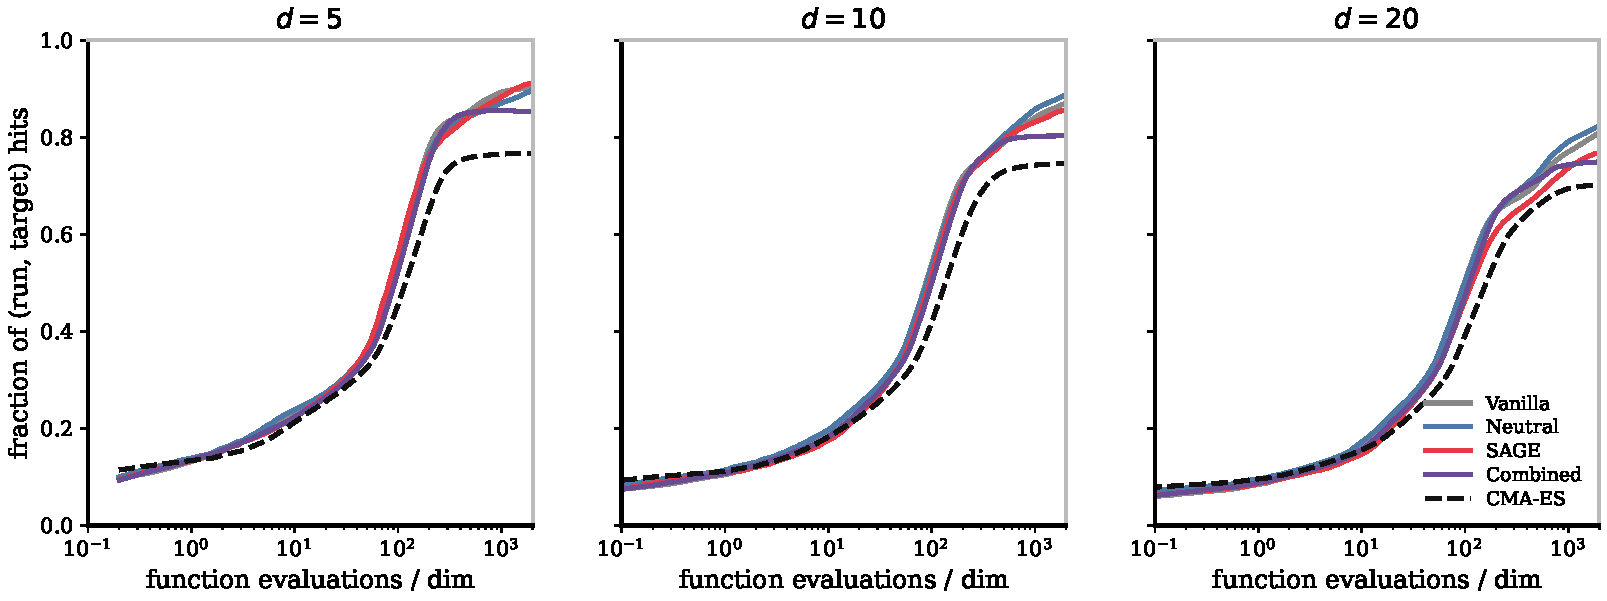
\includegraphics[width=\textwidth]{figures/fig_phase4_fullsuite_ecdf.pdf}
  \caption{Empirical attainment function (EAF) on the full $1{,}000$-instance MA-BBOB pool at $d \in \{5, 10, 20\}$. Each curve aggregates 51 log-spaced fitness targets in $[10^{-8}, 10^2]$ across $5{,}000$ runs per algorithm; the y-axis reports the fraction of (run, target) pairs satisfied by a given function-evaluation budget. Top row: full $[0, 1]$ EAF range. Bottom row: zoomed to $[0.6, 1]$ to resolve the plateau differences between algorithms. The dashed line marks the external CMA-ES baseline; the four LLM-generated variants overlap to within line-width and sit above it by a stable margin throughout the budget.}
  \label{fig:phase4-fullsuite-ecdf}
\end{figure*}

\Cref{tab:phase4-fullsuite-summary} reports the mean AOCC per (algorithm, dimensionality) cell. Three observations follow. First, all four LLM-generated algorithms beat the CMA-ES baseline by a margin of $0.10$--$0.12$ mean AOCC, uniformly across $d \in \{5, 10, 20\}$. The smallest gap, $0.10$ at $d = 20$, is still larger by an order of magnitude than the $0.022$--$0.023$ within-condition spread observed in the head-to-head comparison of \cref{sec:results-stage4-agg}. Second, the ranking within the LLM group is nearly indistinguishable: \texttt{IGA\_CMA} (vanilla) narrowly leads at $d = 5$ at $0.848$, while \texttt{BIPOP\_MA\_CMA\_ES} (neutral) takes the lead at $d = 10$ ($0.810$) and $d = 20$ ($0.745$). The total spread among the four LLM winners is $0.03$--$0.05$ AOCC across the three dimensionalities --- close to the noise floor implied by the heavy-tailed per-instance AOCC distributions. Third, the head-to-head winner of \cref{sec:results-stage4-agg} (combined) does not reproduce its lead on the broader benchmark: it ranks fourth at $d = 5$, third at $d = 10$, and second at $d = 20$. The $0.022$--$0.023$ AOCC advantage of the combined condition observed on the twenty-function set therefore does not transfer to the full pool.

\Cref{fig:phase4-fullsuite-ecdf} extends the same observations onto the per-FE attainment dimension. The CMA-ES baseline tracks the LLM variants closely through the early budget but separates from them past the mid-budget mark, where the LLM variants' final-stage exploitation pays off. The four LLM ECDF curves themselves are visually indistinguishable across all three dimensionalities: the within-LLM ranking that \cref{sec:results-stage4-agg} relies on is not stable under generalisation.

The implication for the thesis claims is two-sided. On the one hand, the mainline narrative --- that the LLM-generated CMA-ES variants are good optimisers on this benchmark family --- holds robustly: every winner beats the canonical CMA-ES on the full $1{,}000$-instance pool, at every tested dimensionality, and by a margin that swamps any within-LLM ranking. On the other hand, the per-condition ranking observed in \cref{sec:results-stage4-agg} is not stable when re-evaluated on the broader benchmark: the $0.022$--$0.023$ AOCC gap between vanilla, neutral, sage, and combined that is detectable on twenty functions disappears into the noise floor on $1{,}000$. The feedback string that produced each winner therefore matters for which CMA-ES decoration the LLM bolts on (\cref{sec:results-stage4-winners}), but not measurably for the algorithm's broad-benchmark performance.